\documentclass[
	parspace, % Add vertical space between paragraphs
	%noindent, % No indentation of first lines in each paragraph
	%nohyp, % No hyphenation of words
	%twoside, % Double sided format
	%draft, % Quicker draft compilation without rendering images
	%final, % Set final to hide todos
]{elteikthesis}[2024/04/26]

% Document's metadata
\title{Web alapú deep learning szolgáltatás vadállatok felismerésére}
\date{2026}

% Author's metadata
\author{Mihályi Dániel Attila}
\degree{programtervező informatikus BSc}

% Superivsor(s)' metadata
\supervisor{Dobos László} % internal supervisor's name
\affiliation{Egyetemi Adjunktus}
\extsupervisor{Dudás Bence} % external supervisor's name
\extaffiliation{doktorandusz}

% University's metadata
\university{Eötvös Loránd Tudományegyetem}
\faculty{Informatikai Kar}
\department{Programozáselmélet és Szoftvertechnológiai \\ Tanszék}
\city{Budapest}
\logo{elte_cimer_szines}

% Add bibliography file
\addbibresource{elteikthesis.bib}

\begin{document}

\documentlang{hungarian}

% Címlap
\maketitle

% Tartalomjegyzék
\tableofcontents
\cleardoublepage

% ----------------------------------------------------------------------------
\chapter{Bevezetés}
\label{ch:intro}

A természetvédelmi kutatások egyik legkritikusabb szakasza a terepi adatgyűjtés és az azt követő feldolgozás. A vadon élő állatok megfigyelése során keletkező hatalmas mennyiségű képi anyag manuális osztályozása rendkívül lassú és fáradságos munka. Jelen dolgozat egy olyan megoldást mutat be, amely modern webtechnológiák és a mesterséges intelligencia ötvözésével automatizálja ezt a munkafolyamatot.

\section{Motiváció és Problémafelvetés}
A kutatók számára gyakran problémát jelent az adatok központosított tárolása és a helyszíni megfigyelések pontos geolokációs rögzítése. Egy olyan rendszerre van szükség, amely:
\begin{itemize}
    \item Azonnali visszajelzést ad az állatfajról a terepen készült fotó alapján.
    \item Biztosítja a megfigyelések térképes vizualizációját.
    \item Biztonságosan tárolja a felhasználók adatait és feltöltéseit.
    \item Könnyen telepíthető és hordozható különböző szerverkörnyezetek között.
\end{itemize}

\section{Választott technológiák}
A választott stack alapvető célja a gyors fejleszthetőség és a stabilitás volt.
\begin{itemize}
    \item \textbf{Python Dash:} A frontend és backend közötti szoros integrációt biztosítja, lehetővé téve komplex reaktív felületek létrehozását tiszta Python kóddal \cite{dash_docs}.
    \item \textbf{Supabase:} Egy nyílt forráskódú "Firebase alternatíva", amely a PostgreSQL-re építve biztosítja az autentikációt és az adatbázis-kezelést. A projekt során a Supabase \textbf{önkiszolgáló (self-hosted)} változatát alkalmaztam Docker környezetben, ami teljes kontrollt biztosít az adatok felett \cite{supabase_docs}.
    \item \textbf{TensorFlow/Keras:} A mélytanulási modell futtatásáért és a predikciókért felelős \cite{tensorflow_docs}.
    \item \textbf{Docker:} A mikroszolgáltatás-alapú architektúra izolációját és hordozhatóságát garantálja \cite{docker_docs}.
\end{itemize}

\chapter{Felhasználói dokumentáció}
\label{ch:user}

\section{A szoftver célja és ismertetése}
A Vadvilág Dashboard egy olyan döntéstámogató rendszer, amely mesterséges intelligencia segítségével segíti a kutatók munkáját. A szoftver automatikusan azonosítja a terepi fotókon látható vadállatokat, és lehetőséget biztosít az észlelések földrajzi rögzítésére és térképes vizualizációjára.

\section{Célközönség}
A rendszer elsősorban terepi kutatók, ökológusok és természetvédelmi szakemberek számára készült, akik nagy mennyiségű vadkamerás felvételt dolgoznak fel, és szükségük van a megfigyelések központosított, térképalapú kezelésére.

\section{Rendszerkövetelmények}
A szoftver futtatásához az alábbi minimális és optimális környezet szükséges:
\begin{itemize}
    \item \textbf{Minimális HW/SW környezet:}
    \begin{itemize}
        \item Docker Desktop vagy Docker Compose (V2).
        \item 4 GB RAM, 2 magos CPU.
        \item Webböngésző (Chrome, Firefox vagy Edge).
    \end{itemize}
    \item \textbf{Optimális HW/SW környezet:}
    \begin{itemize}
        \item 8 GB RAM (a modell gyorsabb betöltése és futtatása érdekében).
        \item 4+ magos processzor.
        \item Stabil internetkapcsolat (elsősorban a Docker image-ek letöltéséhez és a demó eléréséhez).
    \end{itemize}
\end{itemize}

\section{Üzembe helyezés és indítás}
A telepítési útmutató a valóságos, Docker-alapú folyamatot követi:
\begin{enumerate}
    \item Töltse le a projekt forráskódját.
    \item Nyisson terminált a projekt \texttt{src/} könyvtárában, és adja ki a \texttt{docker compose up -{}-build} parancsot.
    \item A konténerek elindulása után az alkalmazás a \texttt{http://localhost:8050} címen érhető el.
\end{enumerate}
A nyilvános demó változat elérhetősége: \url{https://huggingface.co/spaces/Micsu0930/Vadvilag_Dashboard}.

\section{Általános felhasználói tájékoztató}
Az alkalmazás kezelése szabványos böngésző alapú interakciókra épül. A térképkezelés a bal egérgombbal (vonszolás, pontválasztás) és a görgővel (zoom) történik. A rendszer reszponzív, így mobil eszközökön is használható a terepen.

\section{A rendszer funkcióinak ismertetése és folyamata}

\subsection{Nyitóoldal és Navigáció}
Az alkalmazás indításakor a nyitóoldal (Landing Page) fogadja a felhasználót (lásd: \ref{fig:landing}. ábra), amely tájékoztat a rendszer képességeiről és a támogatott fajok számáról.

\begin{figure}[H]
    \centering
    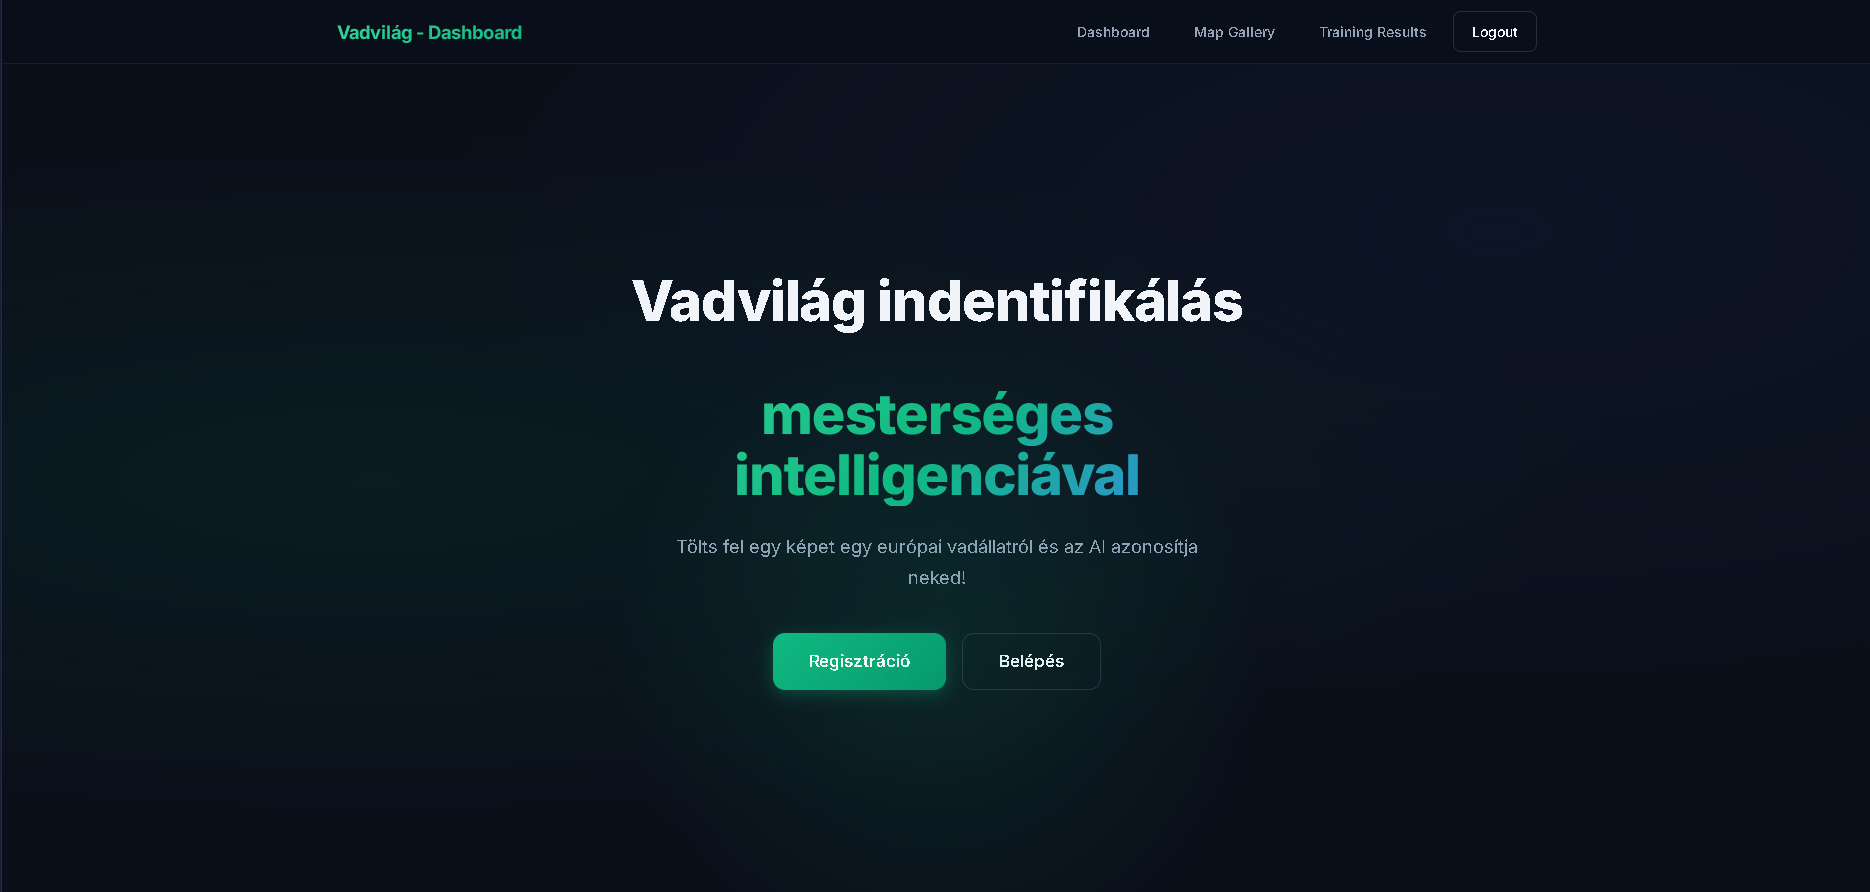
\includegraphics[width=0.85\textwidth]{images/landing_page.png}
    \caption{A rendszer nyitóoldala (Landing Page)}
    \label{fig:landing}
\end{figure}

\subsection{Regisztráció és Belépés}
A funkciók eléréséhez bejelentkezés szükséges. A felhasználók a Supabase Auth segítségével biztonságosan regisztrálhatnak és léphetnek be.

\subsection{Osztályozási munkafolyamat}
A munkafolyamat a központi irányítópulton (Dashboard) zajlik (lásd: \ref{fig:dashboard}. ábra):
\begin{enumerate}
    \item \textbf{Helyszínválasztás:} Kattintással jelölje meg a fotó készítésének helyét a térképen.
    \item \textbf{Feltöltés:} Válassza ki vagy húzza be a fotót.
    \item \textbf{Eredmény:} A rendszer megjeleníti a faj nevét és a konfidencia szintet, majd az adatokat menti az adatbázisba.
\end{enumerate}

\begin{figure}[H]
    \centering
    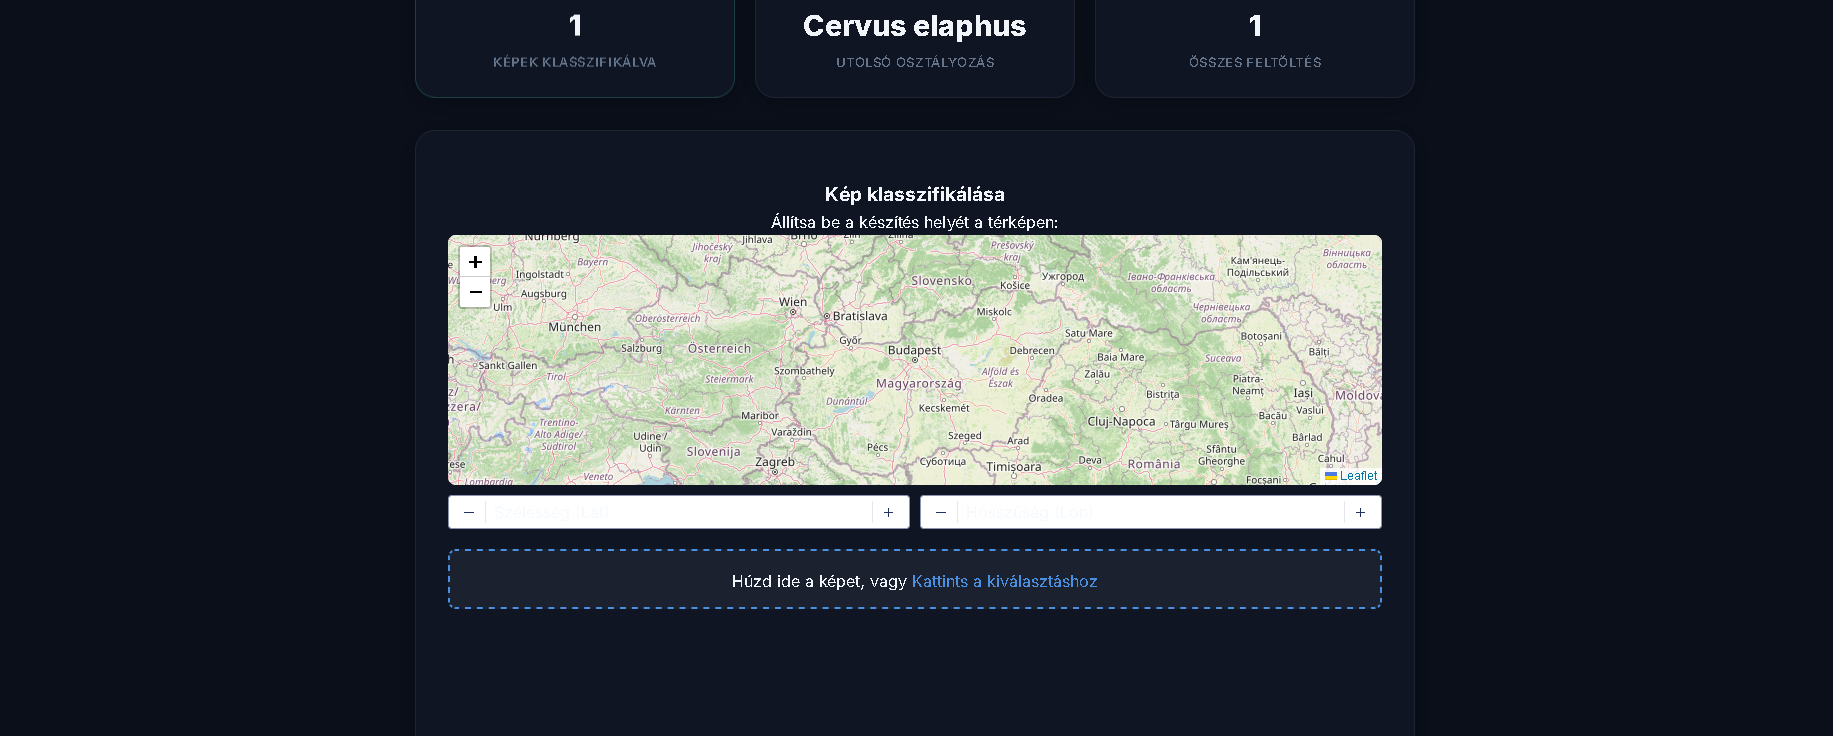
\includegraphics[width=0.85\textwidth]{images/dashboard_main.png}
    \caption{A központi klasszifikációs irányítópult}
    \label{fig:dashboard}
\end{figure}

\subsection{Adatok vizualizációja}
A rögzített adatok a "Map Gallery" menüpontban tekinthetők meg (lásd: \ref{fig:gallery}. ábra). A térképen lévő jelölőkre kattintva a jobb oldali panelen láthatóvá válik a rögzített fotó és az észlelés összes adata.

\begin{figure}[H]
    \centering
    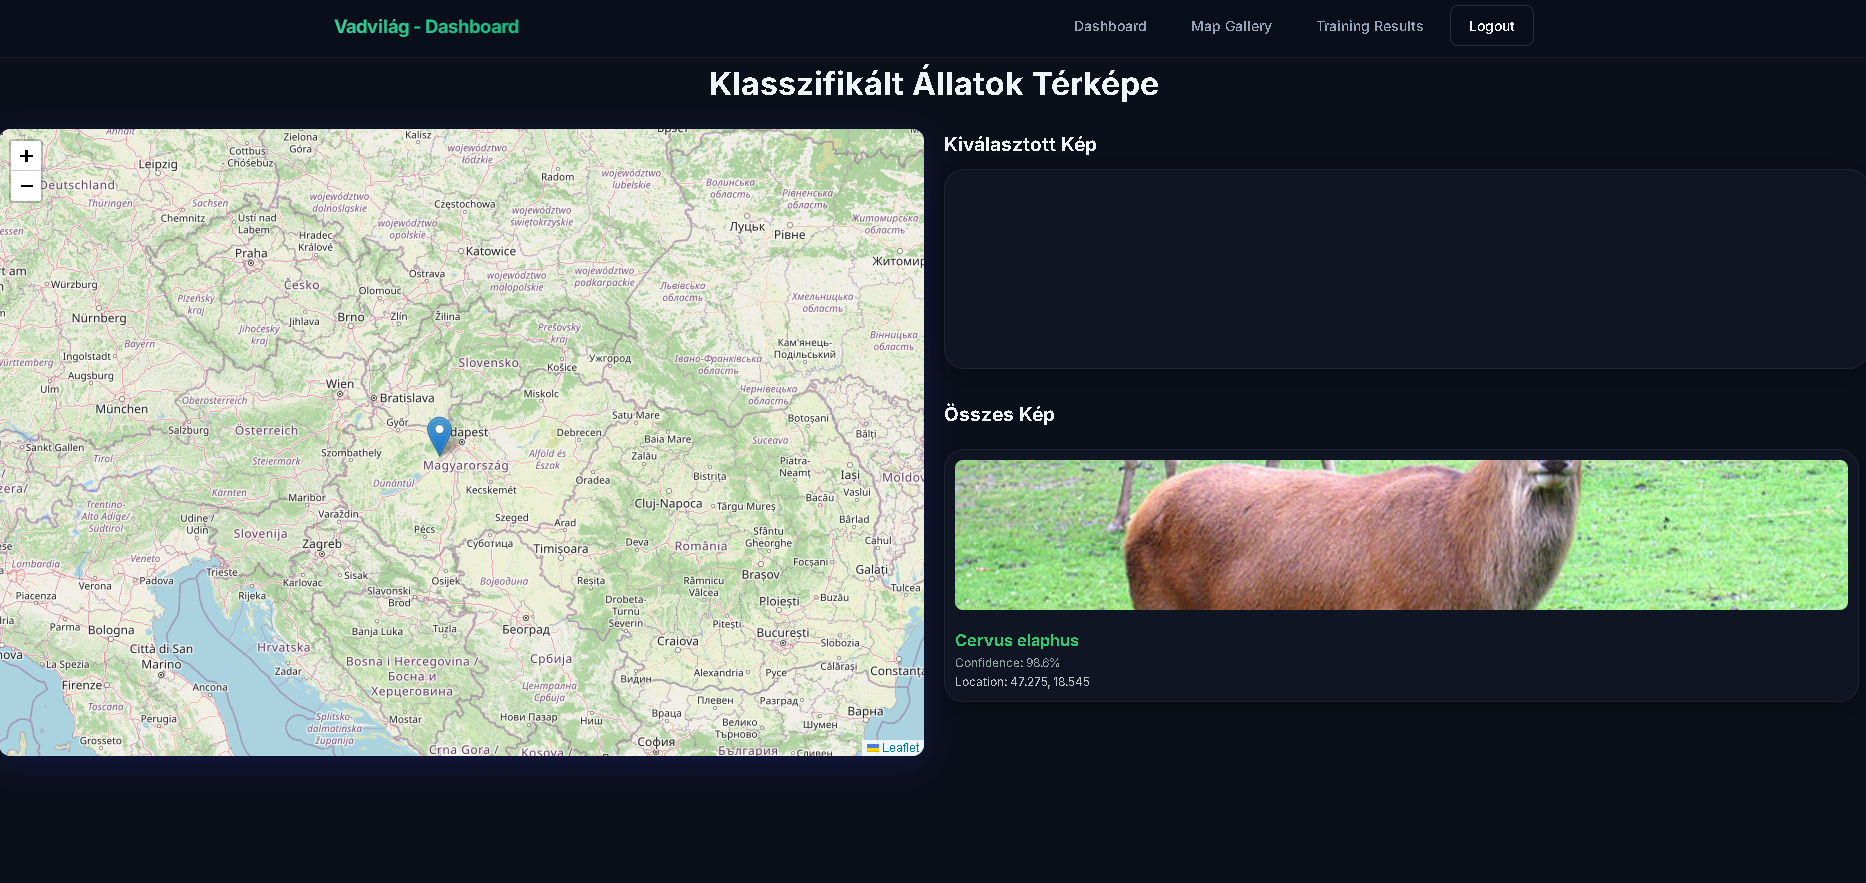
\includegraphics[width=0.85\textwidth]{images/map_gallery_view.png}
    \caption{Interaktív térkép és galéria nézet}
    \label{fig:gallery}
\end{figure}

\section{Rendszerüzenetek és Hibaelhárítás}
\begin{itemize}
    \item \textbf{Hibaüzenetek:}
    \begin{itemize}
        \item \textit{"Invalid credentials"}: Hibás belépési adatok. Megoldás: ellenőrizze az emailt/jelszót.
        \item \textit{"Hiányzó koordináta"}: Nem választott helyszínt. Megoldás: kattintson a térképre a feltöltés előtt.
        \item \textit{"A Tensorflow nem tölthető be"}: Memória hiba a Docker konténerben. Megoldás: növelje a Docker számára kiosztott RAM mennyiségét.
    \end{itemize}
    \item \textbf{Biztonsági előírások:} A felhasználói adatokat a PostgreSQL RLS (Row Level Security) védi, így mindenki csak a saját észleléseit szerkesztheti.
\end{itemize}

\begin{figure}[H]
    \centering
    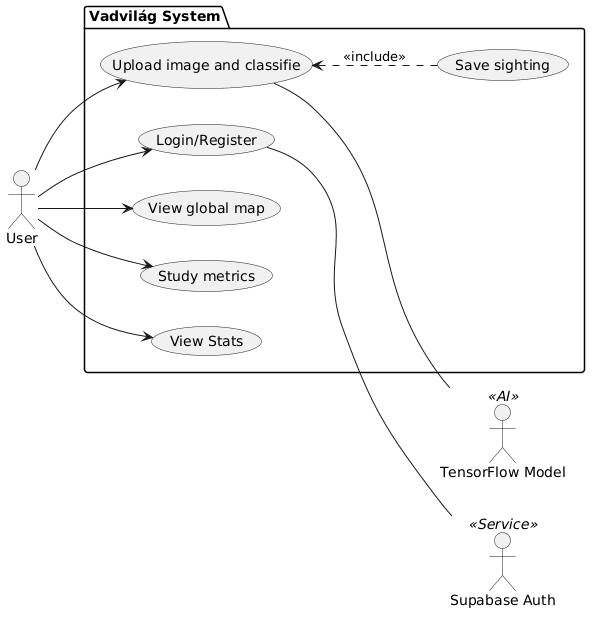
\includegraphics[width=0.7\textwidth]{images/use_case_diagram.png}
    \caption{A rendszer használati esetei (Use Case)}
    \label{fig:use-case-user}
\end{figure}


\chapter{Fejlesztői dokumentáció}
\label{ch:dev-doc}
Ez a fejezet a rendszer technikai megvalósítását, az architektúra tervezését és az alkalmazott algoritmusok részleteit mutatja be fejlesztői szemszögből.

\section{Specifikáció és Tervezés}
\label{sec:design}
A fejlesztési folyamat első lépése a követelmények pontos meghatározása és a rendszerszintű tervezés volt, biztosítva a megoldandó probléma hatékony technikai leképezését.

\subsection{Használt fogalmak és technológiák definíciója}
A dolgozatban alkalmazott kulcsfogalmak és technológiák meghatározása az alábbi:
\begin{itemize}
    \item \textbf{Mesterséges Intelligencia (MI):} A számítástechnika azon ága, amely olyan rendszerek létrehozásával foglalkozik, amelyek képesek az emberi intelligenciát igénylő feladatok (például vizuális felismerés, döntéshozatal vagy komplex mintafelismerés) elvégzésére.
    \item \textbf{Gépi Tanulás (Machine Learning):} Az MI egy részterülete, amely olyan algoritmusokra összpontosít, amelyek explicit programozás nélkül, tapasztalati adatokból tanulva képesek mintázatok felismerésére és előrejelzések készítésére.
    \item \textbf{Neurális Hálózatok (Neural Networks):} Olyan gépi tanulási modellek, amelyeket az emberi agy biológiai neuronhálózatának szerkezete és működése ihletett. Egymáshoz kapcsolódó rétegekből és csomópontokból állnak, amelyek súlyozott kapcsolatokon keresztül dolgozzák fel az információt.
    \item \textbf{Mély Tanulás (Deep Learning):} Olyan neurális hálózatok, amelyek számos (akár több száz) rejtett rétegből állnak. Ez a technológia teszi lehetővé a komplex, strukturálatlan adatok — például képek — nagy pontosságú elemzését, ahogy azt a projektben használt ConvNeXt architektúra is teszi.
    \item \textbf{Klasszifikáció (Osztályozás):} Az a folyamat, amely során a bemeneti adatokat (képeket) előre meghatározott kategóriákba (állatfajok) soroljuk.
    \item \textbf{Docker konténerizáció:} Szoftvercsomagolási technológia, amely lehetővé teszi az alkalmazás és függőségeinek izolált futtatását bármilyen környezetben.
    \item \textbf{Single Page Application (SPA):} Olyan webalkalmazás, amely egyetlen HTML oldal betöltése után dinamikusan frissíti a tartalmát, folyamatosabb felhasználói élményt nyújtva.
    \item \textbf{Row Level Security (RLS):} Adatbázis-szintű biztonsági mechanizmus, amely rekord-szinten korlátozza a hozzáférést a felhasználói azonosító alapján.
\end{itemize}

\subsection{Részletes funkcionális és nem-funkcionális specifikáció}
A rendszernek az alábbi követelményeket kell teljesítenie:
\begin{itemize}
    \item \textbf{Funkcionális követelmények:}
    \begin{itemize}
        \item Biztonságos felhasználói regisztráció és belépés.
        \item Földrajzi koordináták megadása interaktív térképen.
        \item Képek feltöltése és automatikus fajmeghatározása legalább 65\%-os pontossággal.
        \item Az észlelések térképes és galéria-alapú vizualizációja.
        \item Egyéni felhasználói statisztikák folyamatos frissítése.
    \end{itemize}
    \item \textbf{Nem-funkcionális követelmények:}
    \begin{itemize}
        \item \textbf{Hordozhatóság:} A rendszernek Docker környezetben operációs rendszertől függetlenül működnie kell.
        \item \textbf{Válaszidő:} Az osztályozási folyamatnak (feltöltéstől az eredményig) 3 másodpercen belül le kell futnia.
        \item \textbf{Adatbiztonság:} A felhasználók nem láthatják és nem módosíthatják egymás feltöltéseit.
    \end{itemize}
\end{itemize}

\subsection{Rendszerarchitektúra és rétegek}
Az alkalmazás három jól elkülöníthető rétegre tagozódik:
\begin{itemize}
    \item \textbf{Prezentációs réteg (Frontend):} A Dash keretrendszer által kiszolgált reaktív webes felület, amely HTML5, CSS3 és JavaScript (Plotly) elemekből áll. Ez felelős a felhasználói interakciókért és az adatok vizuális megjelenítéséért.
    \item \textbf{Logikai réteg (Backend):} A Python nyelven írt üzleti logika, amely kezeli a hitelesítést, a képfeldolgozási folyamatokat, az MI modell futtatását (TensorFlow) és az adatok validálását.
    \item \textbf{Adatforrás réteg (Database):} A helyileg futtatott Supabase infrastruktúra (PostgreSQL, GoTrue, PostgREST), amely tárolja a felhasználói profilokat, az észlelések metaadatait és a bináris képkódokat.
\end{itemize}

\subsection{Adatbázis terv és mezőszerkezet}
A rendszer az adatbázis-szintű biztonságot részesíti előnyben a Row Level Security (RLS) segítségével. Az adatok két fő táblában tárolódnak.

\subsubsection{user\_uploads tábla}
Ez a tábla tárolja a rögzített vadállat észlelések minden adatát.
\begin{table}[H]
\centering
\begin{tabular}{|l|l|l|}
\hline
\textbf{Mezőnév} & \textbf{Típus} & \textbf{Leírás} \\ \hline
id & UUID (PK) & Az észlelés egyedi azonosítója. \\ \hline
user\_id & UUID (FK) & A feltöltő felhasználó azonosítója (auth.users). \\ \hline
image\_data & TEXT (Base64) & A feltöltött kép kódolt adatai. \\ \hline
latitude & DECIMAL & A megfigyelés földrajzi szélessége. \\ \hline
longitude & DECIMAL & A megfigyelés földrajzi hosszúsága. \\ \hline
predicted\_class & VARCHAR & Az MI által meghatározott faj neve. \\ \hline
confidence & FLOAT & A predikció valószínűségi értéke (0-1). \\ \hline
created\_at & TIMESTAMP & A rögzítés időpontja. \\ \hline
\end{tabular}
\caption{A user\_uploads tábla szerkezete}
\end{table}

\subsubsection{user\_stats tábla}
A felhasználók összesített statisztikáit tartalmazó tábla a gyors lekérdezés érdekében.
\begin{table}[H]
\centering
\begin{tabular}{|l|l|l|}
\hline
\textbf{Mezőnév} & \textbf{Típus} & \textbf{Leírás} \\ \hline
user\_id & UUID (PK, FK) & A felhasználó egyedi azonosítója. \\ \hline
total\_classified & INTEGER & Az összesített osztályozások száma. \\ \hline
last\_class & VARCHAR & Az utoljára azonosított faj neve. \\ \hline
updated\_at & TIMESTAMP & Az utolsó frissítés időpontja. \\ \hline
\end{tabular}
\caption{A user\_stats tábla szerkezete}
\end{table}

Az adatbázis kapcsolatokat és az RLS szabályokat az ER-diagram (\ref{fig:er}. ábra) szemlélteti. Az RLS biztosítja, hogy a \texttt{SELECT} és \texttt{INSERT} műveletek csak a hitelesített tulajdonos számára legyenek engedélyezettek.

\subsection{Konténerizált architektúra}
A rendszer hét különálló konténerből áll, amelyeket Docker Compose koordinál:
\begin{itemize}
    \item \texttt{wildlife-dashboard}: A fő alkalmazás konténere.
    \item \texttt{wildlife-tensorboard}: A tanítási naplók megjelenítése.
    \item \texttt{supabase-db}: PostgreSQL adatbázis.
    \item \texttt{supabase-auth}: GoTrue alapú autentikációs szerver.
    \item \texttt{supabase-rest}: PostgREST interfész.
    \item \texttt{kong}: API gateway és reverse proxy.
\end{itemize}

\subsection{Rendszerarchitektúra}
A rendszer mikro-architektúrája három fő pillérre épül: a Dash keretrendszerben írt frontend-backend egységre, a Docker környezetben lokálisan futtatott Supabase szolgáltatásokra (Auth és PostgreSQL), valamint a TensorFlow alapú osztályozó modulra.

A \ref{fig:component}. ábra mutatja a komponensek közötti függőségeket. A Dash Dashboard központi szerepet tölt be: kezeli a felhasználói interakciókat, hívja a hitelesítési modult, és továbbítja a képeket az MI processzornak. Az adatok perzisztenciáját a Supabase PostgREST interfészén keresztül a PostgreSQL adatbázis biztosítja \cite{postgrest_docs}.

\begin{figure}[H]
    \centering
    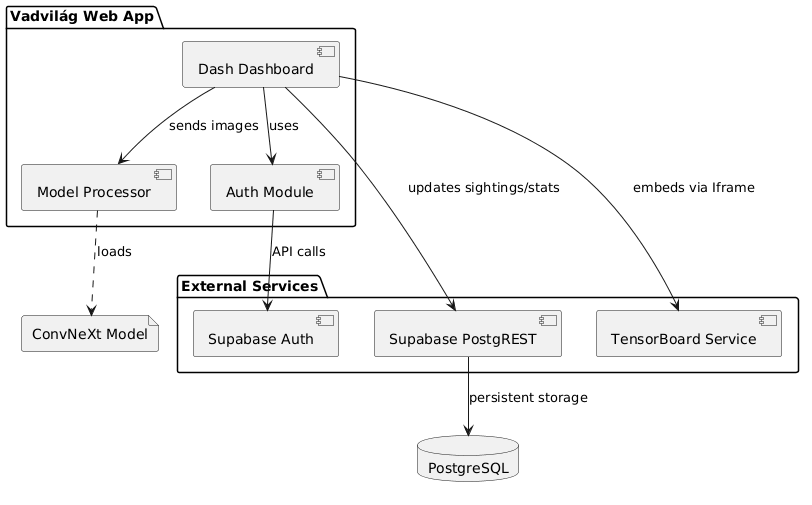
\includegraphics[width=0.9\textwidth]{images/component_diagram.png}
    \caption{A rendszer komponens-szintű architektúra diagramja}
    \label{fig:component}
\end{figure}

A szoftver belső szerkezete (lásd: \ref{fig:package}. ábra) moduláris. A \texttt{src/app} mappában található a logikai mag, ahol a \texttt{pages/} könyvtár tartalmazza az egyes aloldalak (Dashboard, Térkép, Tanítási naplók) implementációját, míg az \texttt{auth.py} a Supabase integrációért felelős.

\begin{figure}[H]
    \centering
    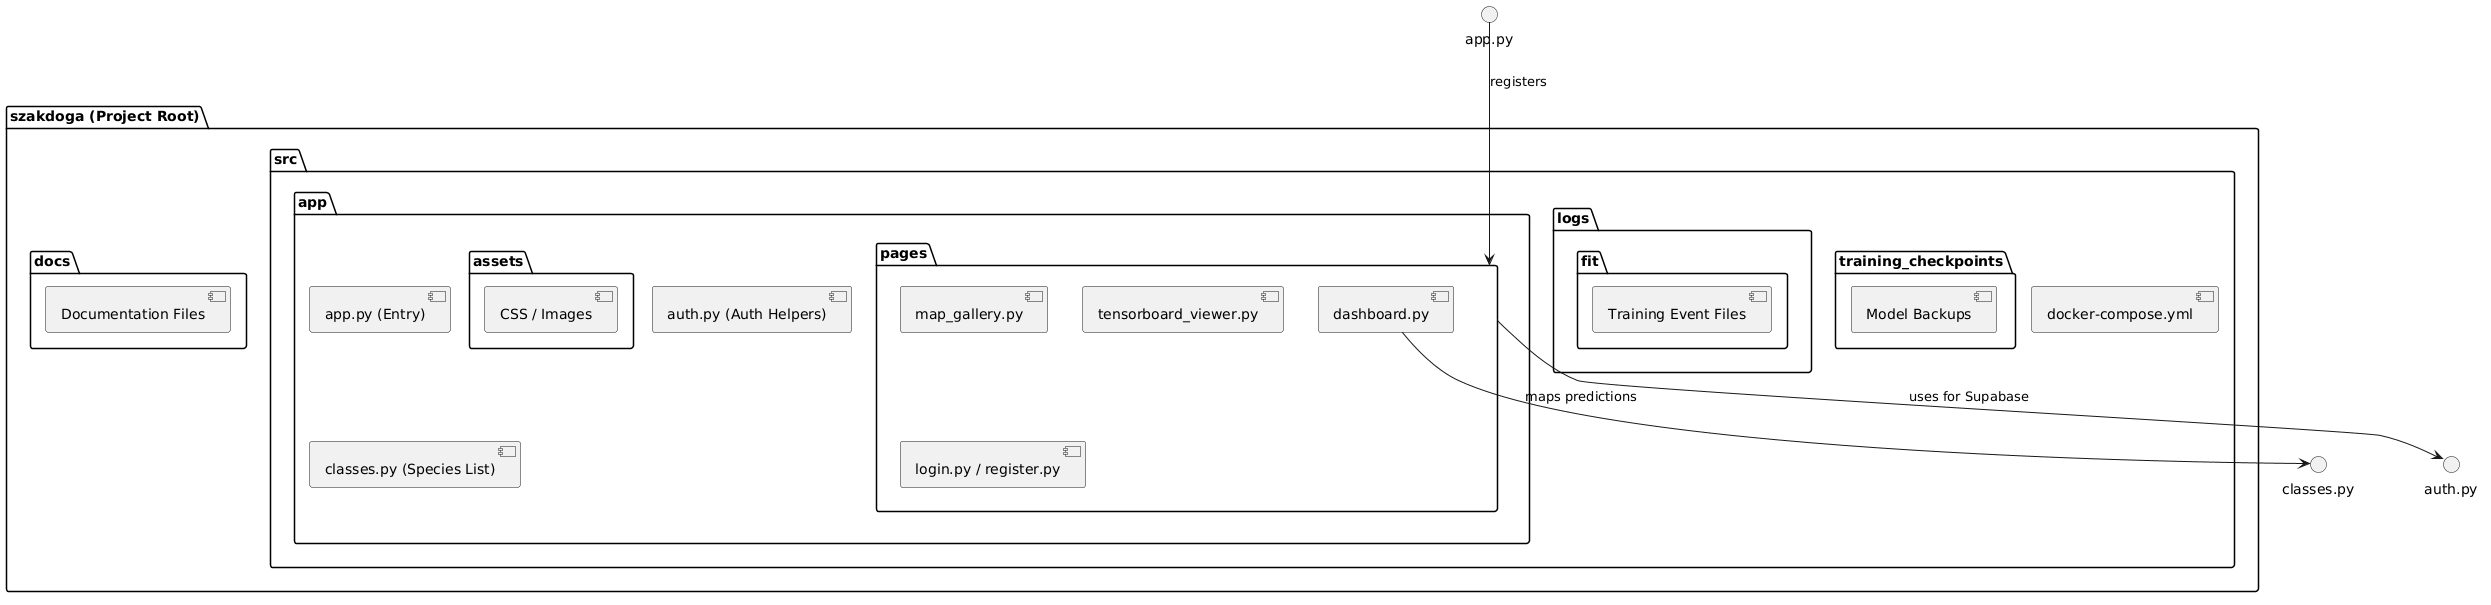
\includegraphics[width=0.7\textwidth]{images/package_diagram.png}
    \caption{A projekt forráskódjának csomag-szintű felépítése}
    \label{fig:package}
\end{figure}

\subsection{Az adatmodell és Biztonság}
Az alkalmazás adatbázis-sémája három fő táblára fókuszál: a hitelesített felhasználókra, az általuk feltöltött képi adatokra és koordinátákra, valamint az összesített statisztikákra.

Az \ref{fig:er}. ábrán látható módon minden feltöltés egy egyedi felhasználóhoz (\texttt{user\_id}) kötődik. Az adatok védelméről a PostgreSQL RLS (Row Level Security) szabályai gondoskodnak, megakadályozva, hogy a felhasználók hozzáférjenek egymás privát adataihoz.

\begin{figure}[H]
    \centering
    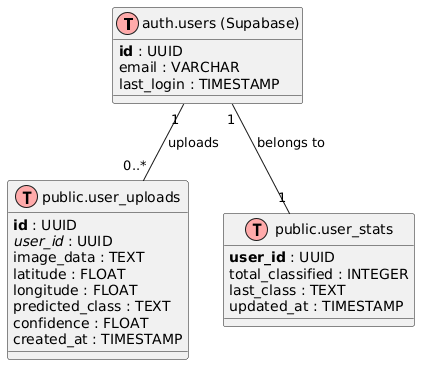
\includegraphics[width=0.6\textwidth]{images/er_diagram}
    \caption{Entitás-kapcsolat (ER) diagram}
    \label{fig:er}
\end{figure}

\subsection{Folyamatvezérlés}
A rendszer legösszetettebb folyamata a képfeltöltés és az automatikus fajmeghatározás, amely több aszinkron lépésből áll.

A \ref{fig:sequence}. ábra részletezi ezt az üzenetváltási folyamatot. A felhasználó feltölti a képet, amit a back-end validál a Supabase Auth segítségével. Sikeres hitelesítés után a ConvNeXt modell elvégzi az inferenciát, majd az eredményt (fajnév és konfidencia szint) a rendszer elmenti az adatbázisba, és frissíti a felhasználó globális statisztikáit.

\begin{figure}[H]
    \centering
    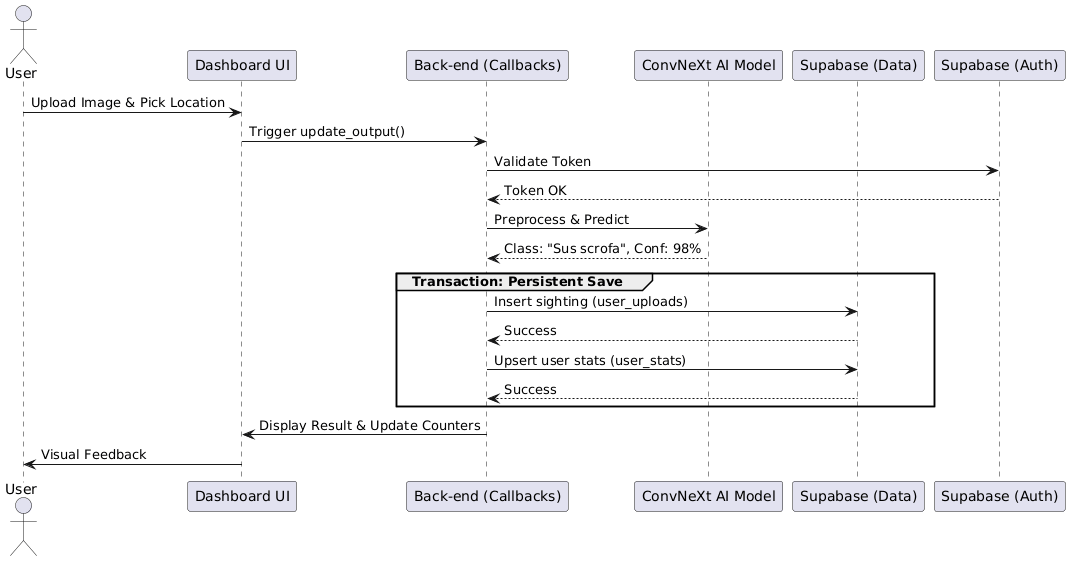
\includegraphics[width=0.8\textwidth]{images/sequence_diagram}
    \caption{Képfeltöltési és osztályozási folyamat szekvencia diagramja}
    \label{fig:sequence}
\end{figure}

\subsection{Infrastruktúra és Hálózat}
A hordozhatóság és a könnyű skálázhatóság érdekében a teljes stack Docker konténerekben fut. A \ref{fig:deployment}. ábrán látható a konténerek elrendezése. A \texttt{wildlife-dashboard} és a \texttt{supabase-db} elkülönített hálózaton kommunikálnak, míg a gazda gép könyvtárai (logs, checkpoints) köteteken keresztül vannak becsatolva.

\begin{figure}[H]
    \centering
    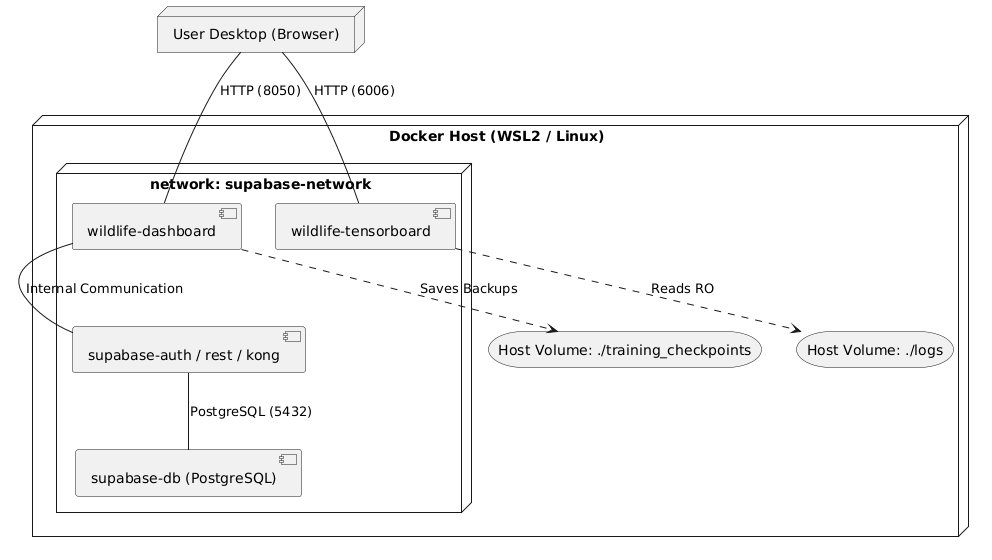
\includegraphics[width=0.8\textwidth]{images/deployment_diagram}
    \caption{Telepítési (Deployment) diagram Docker környezetben}
    \label{fig:deployment}
\end{figure}

A hálózati architektúra (lásd: \ref{fig:network}. ábra) elválasztja a külső elérést a belső szerviz-kommunikációtól. A külső felhasználók a 8050-es (Dashboard) és 6006-os (TensorBoard) portokon érik el a szolgáltatásokat.

\begin{figure}[H]
    \centering
    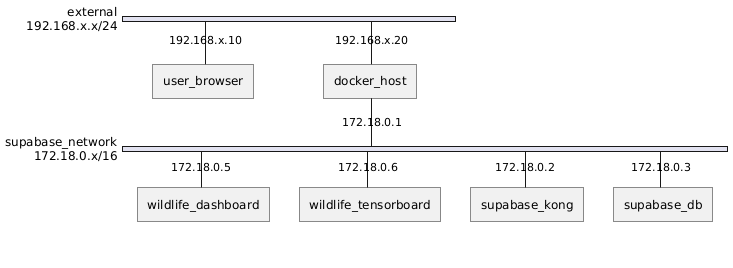
\includegraphics[width=0.8\textwidth]{images/network_diagram}
    \caption{Logikai hálózati struktúra}
    \label{fig:network}
\end{figure}

\section{Implementáció részletei}
\label{sec:impl}
Ez a fejezet a forráskód belső logikáját, a modulok közötti interakciókat és a felhasználói felület technikai megvalósítását részletezi.

\subsection{Modul- és függőségi szerkezet}
Az alkalmazás moduláris felépítésű, ahol az egyes funkcionális egységek (pl. hitelesítés, adatmegjelenítés) különálló fájlokban kaptak helyet. A fontosabb modulok és eljárásaik:

\subsubsection{auth.py - Hitelesítési modul}
Ez a modul felelős a Supabase Auth szolgáltatással való kommunikációért.
\begin{itemize}
    \item \textbf{sign\_in eljárás:}
    \begin{itemize}
        \item \textbf{Bemenet:} Email cím, jelszó.
        \item \textbf{Tevékenység:} Hitelesítési kérést küld a Supabase API-nak.
        \item \textbf{Kimenet:} JWT hozzáférési token vagy hibaüzenet.
    \end{itemize}
    \item \textbf{sign\_up eljárás:}
    \begin{itemize}
        \item \textbf{Bemenet:} Email cím, jelszó.
        \item \textbf{Tevékenység:} Új felhasználó létrehozása az adatbázisban.
        \item \textbf{Kimenet:} Sikerességi állapot és visszaigazoló üzenet.
    \end{itemize}
\end{itemize}

\subsubsection{dashboard.py - Központi logika}
A Dash keretrendszer callback-alapú eseménykezelését valósítja meg.
\begin{itemize}
    \item \textbf{update\_output (Callback):}
    \begin{itemize}
        \item \textbf{Bemenet:} Feltöltött kép (Base64), kiválasztott koordináták (lat, lon).
        \item \textbf{Tevékenység:} Kép előfeldolgozása, MI predikció futtatása, eredmények mentése az adatbázisba.
        \item \textbf{Kimenet:} Frissített UI komponensek (eredmény kártya, statisztikák).
    \end{itemize}
\end{itemize}

\subsection{A felhasználói felület terve és navigáció}
A webes felület tervezésekor a reszponzivitás, az esztétika és az átláthatóság volt az elsődleges szempont. Az alkalmazás tervezése során az alábbi tervezési elveket (UI/UX Principles) követtem:
\begin{itemize}
    \item \textbf{Sötét mód (Dark Mode) alkalmazása:} A sötét háttér és a világos szöveg kontrasztja nemcsak modern esztétikát kölcsönöz, hanem kényelmesebb használatot biztosít alacsony fényviszonyok melletti terepmunka során.
    \item \textbf{Hierarchia és Fókusz:} A legfontosabb funkciókat (térkép, feltöltés) központi helyre, „Glassmorphism” kártyákba rendeztem, hogy a felhasználó figyelme azonnal a lényegi részekre irányuljon.
    \item \textbf{Reszponzivitás:} A CSS Grid és Flexbox technológiák segítségével a felület alkalmazkodik a különböző kijelzőméretekhez (mobil, tablet, asztali gép).
\end{itemize}

Az alkalmazás egy „Single Page Application” (SPA) megközelítést követ a \texttt{dash-pages} segítségével.

\subsubsection{Navigációs struktúra}
A felhasználók közötti navigációt az autentikációs állapot határozza meg (lásd: \ref{fig:authflow}. ábra).
\begin{itemize}
    \item \textbf{Publikus utak:} Kezdőlap (Landing), Belépés, Regisztráció.
    \item \textbf{Védett utak:} Dashboard, Térkép Galéria, TensorBoard nézet.
\end{itemize}
A navigációt egy központi állapotgép vezérli, amely minden oldalváltásnál ellenőrzi a munkamenet érvényességét.

\subsubsection{Eseménykezelés}
A felület interaktivitását a Dash callback mechanizmusa biztosítja. Fontosabb eseménykezelések:
\begin{itemize}
    \item \textbf{Térkép kattintás:} A \texttt{dl.Map} komponens kattintási eseménye frissíti a koordináta beviteli mezőket.
    \item \textbf{Képfeltöltés:} A \texttt{dcc.Upload} eseménye azonnali láncreakciót vált ki, amely magában foglalja az MI elemzést és az aszinkron adatbázis mentést.
\end{itemize}

\begin{figure}[H]
    \centering
    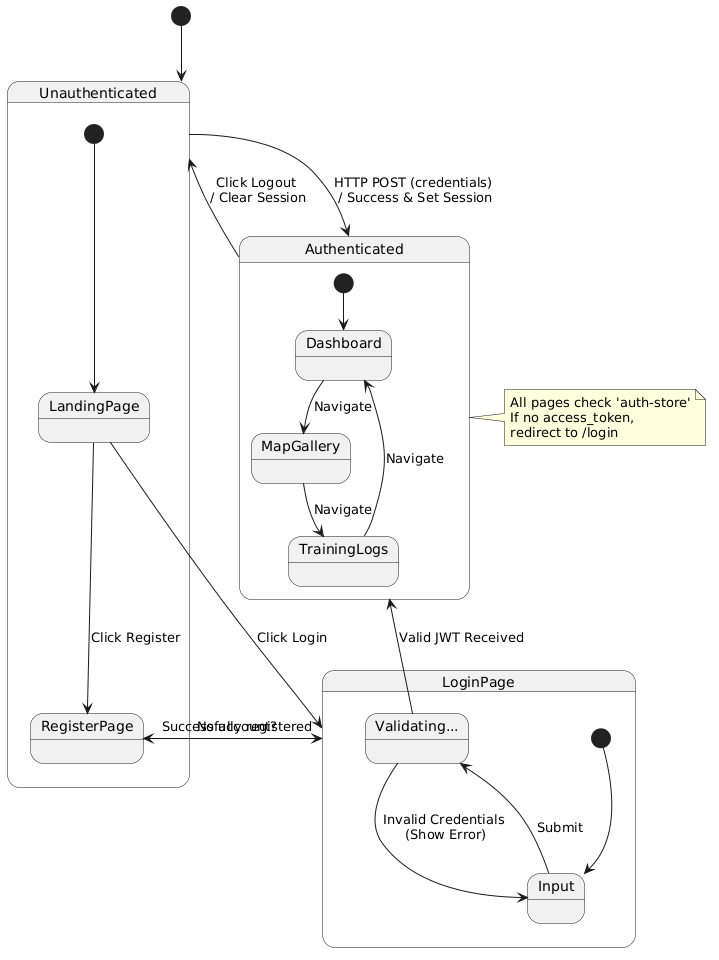
\includegraphics[width=0.7\textwidth]{images/auth_flow_diagram.png}
    \caption{Hitelesítési és navigációs folyamat terve}
    \label{fig:authflow}
\end{figure}

\subsection{Képfeldolgozás és Osztályozás}
A \texttt{dashboard.py}-ban megvalósított \texttt{update\_output} függvény végzi az osztályozás nagy részét:
\begin{enumerate}
    \item \textbf{Dekódolás:} A Base64 kódolt képet \texttt{io.BytesIO} segítségével alakítjuk át.
    \item \textbf{Előfeldolgozás:} A \texttt{PIL.Image} könyvtárral $224 \times 224$ képpontos méretre méretezzük át a fotót, ami a ConvNeXtBase modell bemeneti elvárása.
    \item \textbf{Inferencia:} A \texttt{tensorflow.keras.models.load\_model} hívással betöltött modell lefuttatja a predikciót a normalizált \texttt{numpy} tömbön.
    \item \textbf{Leképzés:} A kapott indexet a \texttt{classes.py}-ban található 594 elemű \texttt{CLASS\_NAMES} lista segítségével fordítjuk le a latin fajnévre.
\end{enumerate}

\subsection{Adatbázis-interakció és Biztonság}
A Supabase kliens inicializálása az \texttt{auth.py} modulban történik a környezeti változókból beolvasott URL és kulcs segítségével. A biztonságot a token-alapú hitelesítés garantálja:
\begin{verbatim}
create_client(url, key, options=ClientOptions(
    headers={'Authorization': f'Bearer {access_token}'}
))
\end{verbatim}
Ez a megközelítés lehetővé teszi, hogy a PostgreSQL szintjén definiált RLS szabályok automatikusan érvényesüljenek, mivel az adatbázis "látja" a bejelentkezett felhasználó azonosítóját a kérés fejlécében.

\section{Megvalósítás és Kódminőség}
\label{sec:implementation-details}
Ez a szakasz a fejlesztés során hozott technikai döntéseket, az alkalmazott kódolási konvenciókat és a szoftver belső minőségét biztosító megoldásokat mutatja be.

\subsection{Programozási nyelv és Nyelvi elemek}
A fejlesztéshez a \textbf{Python 3.10+} nyelvet választottam, mivel ez a platform biztosítja a legszélesebb körű támogatást a gépi tanulási modellekhez és a gyors prototípus-gyártáshoz. A megvalósítás során törekedtem a modern és hatékony nyelvi elemek használatára:
\begin{itemize}
    \item \textbf{Típusjelölések (Type Hinting):} A függvények szignatúrájában alkalmazott típusjelölések (pl. \texttt{access\_token: str}) javítják a kód olvashatóságát és segítik a statikus kódelemző eszközök munkáját.
    \item \textbf{F-stringek:} A karakterláncok formázásához a modern \texttt{f"..."} szintaxist használtam, amely nemcsak olvashatóbb, de futásidőben gyorsabb is, mint a korábbi megoldások.
    \item \textbf{Dekorátorok:} A Dash keretrendszer \texttt{@callback} dekorátorait használtam az eseményvezérelt logika deklaratív leírására, ami tisztán elválasztja a UI-t és az üzleti logikát.
    \item \textbf{Opcionális paraméterek:} A segédfüggvényeknél (pl. \texttt{\_dash\_stat}) alkalmazott alapértelmezett értékek rugalmassá teszik a komponensek újrafelhasználását.
\end{itemize}

\subsection{Kódstruktúra és Olvashatóság}
A forráskód külalakja követi a \textbf{PEP 8} stílusútmutatót. A kód tagolása (bekezdések, üres sorok) segíti a logikai egységek elkülönítését.
\begin{itemize}
    \item \textbf{Névkonvenciók:} Minden azonosító beszédes és konvencionális: a változók és függvények \texttt{snake\_case}, az osztályok \texttt{PascalCase} formátumúak. Például a \texttt{total\_classified} vagy \texttt{get\_supabase\_client} nevek egyértelműen tükrözik a változó vagy függvény célját.
    \item \textbf{Öndokumentáló kód:} A választott azonosítók és a tiszta logika miatt a kód nagyrészt öndokumentáló. Ahol szükséges, ott Google-stílusú docstringekkel láttam el a függvényeket, részletezve a bemeneti paramétereket és a visszatérési értékeket.
    \item \textbf{Modularitás és Újrafelhasználás:} A rendszert modulokra bontottam (\texttt{auth.py}, \texttt{pages/}, \texttt{classes.py}). A UI komponensek ismétlődő részeit (pl. statisztikai kártyák) segédfüggvényekbe szerveztem, elkerülve a kódduplikációt (DRY elv).
\end{itemize}

\subsection{Hibakezelés és Ellenőrzés}
A rendszer robusztusságát kiterjedt hibakezelési mechanizmusok biztosítják:
\begin{itemize}
    \item \textbf{Kivételkezelés:} Minden külső API hívást (Supabase) és modell műveletet \texttt{try-except} blokkokba zártam. Ez megakadályozza az alkalmazás összeomlását hálózati hiba vagy hiányzó fájlok esetén, és lehetőséget ad értelmes hibaüzenetek megjelenítésére a felhasználó felé.
    \item \textbf{Bemeneti validáció:} A feltöltés előtt a rendszer ellenőrzi a szükséges adatok (pl. koordináták) meglétét. Amennyiben ezek hiányoznak, az alkalmazás figyelmezteti a felhasználót, ahelyett, hogy hibás adatokat mentene az adatbázisba.
    \item \textbf{Fokozatos funkcionalitás csökkenés} Ha a TensorFlow modell nem tölthető be (pl. memória hiány miatt), a rendszer nem omlik össze, hanem letiltja a klasszifikációs funkciót, miközben a többi rész (pl. galéria) továbbra is használható marad.
\end{itemize}

\subsection{Hatékonyság és Erőforrás-gazdálkodás}
A szoftver tervezésekor figyelembe vettem a számítási és emberi erőforrások optimalizálását:
\begin{itemize}
    \item \textbf{Adatábrázolás:} A képeket Base64 formátumban kezeljük a memóriában az azonnali megjelenítéshez, de az adatbázisba történő mentés előtt a kliens oldalon validáljuk a méretet. A geolokációs adatokhoz a precíz \texttt{decimal} típust használjuk.
    \item \textbf{Memóriakezelés:} A nagy méretű MI modellt csak az első használatkor töltjük be (Lazy Loading), és globális változóban tároljuk, elkerülve a felesleges újra-betöltéseket minden kérésnél.
    \item \textbf{Kép-előfeldolgozás:} A feltöltött fotókat az inferencia előtt azonnal $224 \times 224$ képpontra méretezzük át, ami drasztikusan csökkenti a neurális hálózat számítási igényét és a memória-lábnyomát.
    \item \textbf{Felhasználói idő:} Az aszinkron callback-ek és a \texttt{dcc.Loading} indikátorok biztosítják, hogy a felhasználó folyamatos visszajelzést kapjon a háttérben zajló folyamatokról, növelve a türelmét és a felhasználói élményt.
\end{itemize}

\subsection{Fizikai komponensek és Telepítés}
Az alkalmazás fizikai komponenseinek kapcsolatrendszerét a mikroszolgáltatás-alapú architektúra határozza meg, amelyet a Docker Compose koordinál.

\begin{itemize}
    \item \textbf{Fizikai izoláció:} Minden komponens (Dashboard, Adatbázis, Autentikációs szerver) különálló Docker konténerben fut, ami biztosítja, hogy a függőségek (pl. a TensorFlow specifikus verziói) ne ütközzenek más rendszerelemekkel.
    \item \textbf{Komponensek kapcsolata:} A konténerek egy belső, izolált virtuális hálózaton (\texttt{wildlife-network}) keresztül kommunikálnak. A Dashboard a Supabase szolgáltatásait a Kong API Gateway-en keresztül éri el, ami egységes belépési pontot és biztonsági réteget biztosít.
    \item \textbf{Telepítés módja:} A rendszer telepítése a \texttt{Infrastructure as Code} elvét követi. A \texttt{Dockerfile} és a \texttt{docker-compose.yml} fájlok tartalmazzák a teljes környezeti konfigurációt, így a telepítés egyetlen paranccsal (\texttt{docker compose up}) elvégezhető bármilyen Docker-képes operációs rendszeren, minimalizálva a manuális konfigurációs hibák lehetőségét.
\end{itemize}

\chapter{MI Modell Tanítása és Matematikai Háttere}
\label{sec:mi-training}
A projekt központi eleme egy mély neurális hálózat, amely a legmodernebb látás alapú technológiákat ötvözi. A fejlesztés során a ConvNeXt architektúrára esett a választás, amely egyfajta hidat képez a klasszikus konvolúciós hálózatok és a modern transzformátor alapú megoldások között.

\section{Elméleti háttér}

\subsection{Konvolúciós Neurális Hálózatok (CNN)}
A konvolúciós neurális hálózatok architektúrája a lokális jellemzők kinyerésére épül. A konvolúciós rétegekben alkalmazott kernelek a bemeneti tenzor felett csúszóablakos módszerrel végzik el a műveleteket, így állítva elő a jellemzőtérképeket (feature maps). A tanítás során ezen szűrők súlyait optimalizáljuk a gradiens alapú hibavisszaterjesztés segítségével, minimalizálva a választott költségfüggvényt (loss function). Ez a struktúra biztosítja a térbeli invarianciát és a hierarchikus jellemző-kinyerést a képi adatokból.

\subsection{Vision Transformerek (ViT) és a ConvNeXt architektúra}
A Vision Transformer (ViT) architektúra az önfigyelmi (self-attention) mechanizmusra épül. A bemeneti képet fix méretű foltokra (patches) bontja, amelyeket beágyazott pozíció-kódolással (positional embedding) ellátott szekvenciális adatként dolgoz fel. Ez a megoldás lehetővé teszi a globális függőségek modellezését a kép teljes területén, szemben a konvolúciók lokális receptív mezőjével.

A projektben alkalmazott \textbf{ConvNeXt} egy modernizált konvolúciós hálózat, amely a klasszikus CNN architektúrák alapjaira építve vezet be optimalizált tervezési megoldásokat. A hálózat felépítésének kulcsfontosságú elemei a nagyobb méretű kernelek, az invertált szűk keresztmetszet (inverted bottleneck) struktúra, a GELU aktivációs függvény, valamint a BatchNorm helyett alkalmazott Layer Normalization (LN). Ezeknek a technikai döntéseknek köszönhetően a ConvNeXt megőrzi a hagyományos konvolúciós műveletek hatékonyságát, miközben reprezentációs képessége a legkorszerűbb modellarchitektúrák szintjére emelkedik.

\section{Matematikai Alapvetések}
A modell rétegei közötti információáramlást alapvetően a konvolúciós művelet határozza meg \cite{hands_on_ml}. Egy $I$ bemeneti képen végzett $K$ kernellel történő konvolúció diszkrét formája:
\begin{equation}
    (I * K)(i, j) = \sum_{m} \sum_{n} I(i+m, j+n) \cdot K(m, n)
\end{equation}
ahol az $i, j$ a kimeneti pixel koordinátái, $m, n$ pedig a kernel indexei. A konvolúciós rétegekben a hálózat párhuzamosan több különböző kernelt használ, amelyek súlyait a kezdetekkor véletlenszerűen inicializáljuk. Ezek a kernelek végigfutnak a bemeneten, és mindegyikük egy-egy új jellemzőtérképet (feature map) hoz létre, amelyeket a következő réteg tovább dolgoz fel. A nagy számú kernel használatának célja, hogy a lehető legtöbb információt kinyerjük a képekből. Bár a betanított hálózatok vizualizációja során megfigyelhető, hogy a korai rétegek gyakran geometriai alakzatokra vagy élekre érzékenyek, a tanítás során nem határozzuk meg előre, hogy egy adott kernel milyen konkrét vizuális jellemzőt erősítsen fel; ezt az elvont reprezentációt a modell teljesen önállóan, az optimalizációs folyamat során alakítja ki.

A ConvNeXt architektúra egyik különlegessége a \textbf{Depthwise Convolution} alkalmazása \cite{convnext_paper}, amely csökkenti a paraméterszámot azáltal, hogy a térbeli és a csatorna-szintű összefüggéseket külön kezeli.

A hálózat nem-linearitását a \textbf{GELU} (Gaussian Error Linear Unit) aktivációs függvény biztosítja, amely a modern Transformer modellekben is elterjedt. Közelítő matematikai alakja:
\begin{equation}
    GELU(x) \approx 0.5x \left( 1 + \tanh \left[ \sqrt{2/\pi} (x + 0.044715x^3) \right] \right)
\end{equation}
Ez a függvény simább gradiensátmenetet tesz lehetővé a ReLU-hoz képest, ami stabilabb tanítást eredményez mély hálózatok esetén \cite{convnext_paper}.

\subsection{Transzfer Tanulás és Finomhangolás}
A projektben a neurális hálózat betanításához a transzfer tanulás (\textit{transfer learning}) módszerét választottam. Ez az eljárás azon az elven alapul, hogy egy nagy, általános adathalmazon (például az ImageNet-en) előtanított modell képességei átvihetők egy új, specifikusabb feladatra. Ahelyett, hogy a hálózatot véletlenszerűen inicializált súlyokkal kezdenénk tanítani, egy olyan modellt veszünk alapul, amely már megtanulta a vizuális jellemzők — például élek, textúrák és összetettebb alakzatok — hatékony felismerését.

A saját implementációmban ez a megközelítés azt jelenti, hogy a választott ConvNeXtBase modell konvolúciós bázisát rögzítettem (\textit{layer freezing}), így az eredeti súlyok nem módosultak a folyamat alatt. A hálózat végére egy egyedi osztályozó réteget (\textit{classification head}) illesztettem, amely a modell által kinyert jellemzőtérképekből (\textit{feature maps}) dolgozva végzi el az állatfajok besorolását. Az egyedi rétegszerkezet az alábbi elemekből épül fel:
\begin{itemize}
    \item \textbf{Global Average Pooling 2D}: A térbeli információk összegzése és a dimenziócsökkentés céljából.
    \item \textbf{Dropout}: 20\%-os rátával a túltanulás megakadályozása érdekében.
    \item \textbf{Dense réteg}: 594 neuronnal (az osztályok számának megfelelően) és Softmax aktivációval a fajok azonosításához.
\end{itemize}
Kizárólag ezeket az újonnan hozzáadott rétegeket tanítottam a saját adathalmazomon, ami jelentősen csökkentette a számítási igényt, és lehetővé tette a pontos osztályozást a rendelkezésre álló tanítóadatok mellett is.

\subsection{Tanítási Folyamat és Optimalizáció}
A modell fejlesztése a \texttt{train\_wildlife\_model.ipynb} notebookban történt. Az adathalmaz forrásaként a GBIF adatbázis szolgált \cite{gbif_data}, amelyből összesen 170\,195 képet használtam fel. Az adatokat 70\% tanító, 15\% validációs és 15\% teszt halmazra osztottam. A feladat egyik legnagyobb kihívását az osztályok közötti egyenlőtlen eloszlás (class imbalance) jelentette, amit a \ref{fig:class_dist}. ábra is jól szemléltet.

\begin{figure}[H]
    \centering
    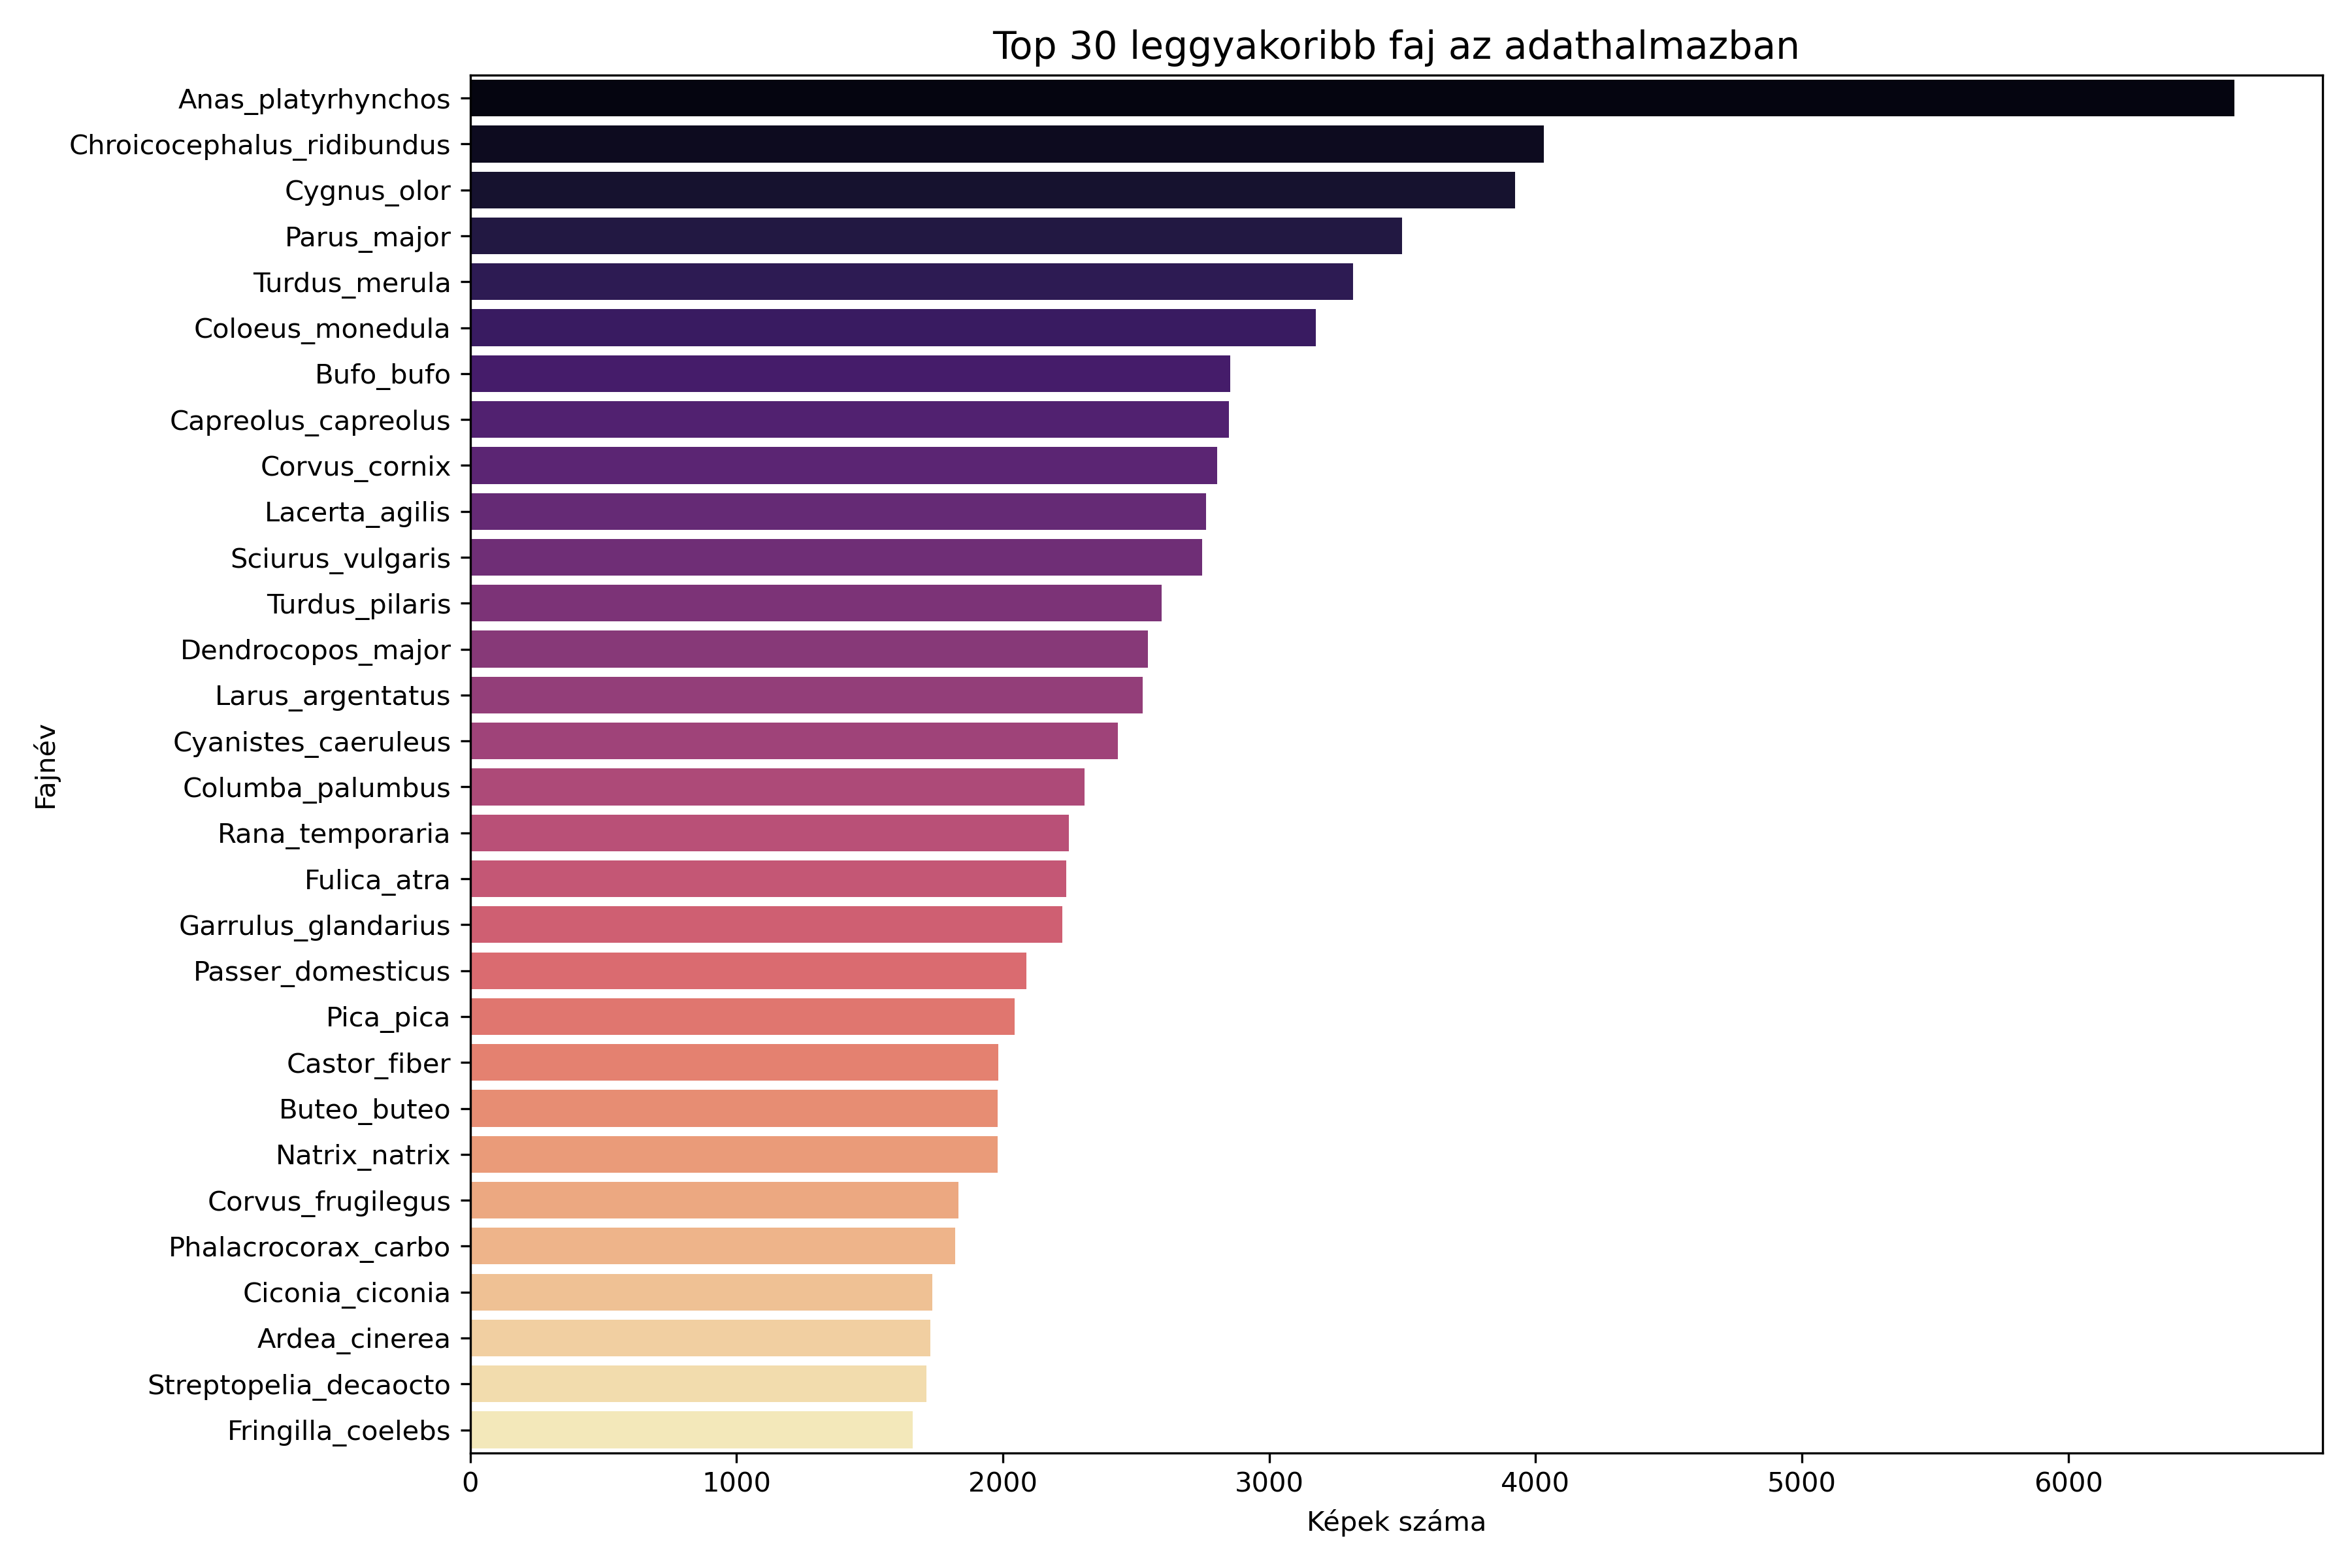
\includegraphics[width=0.9\textwidth]{images/class_dist_top.png}
    \caption{A 15 leggyakoribb faj eloszlása az adathalmazban.}
    \label{fig:class_dist}
\end{figure}

A tanítás során \textbf{Adam} optimalizálót használtam $10^{-3}$ kezdő tanulási rátával. A modell kimeneti rétege egy \textbf{Softmax} függvényt használ, amely a hálózat utolsó rétegének nyers kimeneteit ($z_i$) valószínűségi eloszlássá alakítja:
\begin{equation}
    \sigma(z)_i = \frac{e^{z_i}}{\sum_{j=1}^{K} e^{z_j}}
\end{equation}
ahol $K=594$ a fajok száma. A tanítás során minimalizálandó célfüggvény a \textbf{ritka kategorikus keresztentrópia} (Sparse Categorical Cross-Entropy loss), amely hatékonyabb memóriakezelést tesz lehetővé nagyszámú osztály esetén \cite{hands_on_ml}:
\begin{equation}
    L = -\sum_{i=1}^{K} y_i \log(\hat{y}_i)
\end{equation}
ahol $y_i$ a valódi címke, $\hat{y}_i$ pedig a modell által jósolt valószínűség.

A neurális hálózatok tanítása során alkalmazott visszahívó függvények (callback-ek) olyan segédeszközök, amelyek a tanítási folyamat különböző pontjain — például egy epoch végén vagy egy batch feldolgozása után — automatikusan lefutó kódcsomagok. Ezeket jellemzően a folyamat monitorozására, az állapotok mentésére, vagy a tanítás dinamikus vezérlésére (például idő előtti leállítására) használják. A projekt megvalósításakor az alábbi specifikus callback-eket alkalmaztam a hatékonyság és a folyamat biztonsága érdekében:
\begin{itemize}
    \item \texttt{BackupAndRestore}: Váratlan leállás esetén lehetővé teszi a munka folytatását a legutóbbi sikeres epoch-tól.
    \item \texttt{EarlyStopping}: Megállítja a tanítást, ha a validációs veszteség (\texttt{val\_loss}) már nem javul tovább, elkerülve ezzel a felesleges számítási kapacitás-felhasználást és a túltanulást (a gyakorlatban a tanítás 7 epoch után állt meg).
    \item \texttt{TensorBoard}: Naplózza a metrikákat (veszteség, pontosság), lehetővé téve a tanítási folyamat későbbi vizualizációját és elemzését.
\end{itemize}

A tanítás során rögzített metrikák alapján generált görbéket a \ref{fig:training_curves}. ábra mutatja. Az EarlyStopping mechanizmus sikeresen megakadályozta a túltanulást, a validációs pontosság pedig stabilizálódott.

\begin{figure}[H]
    \centering
    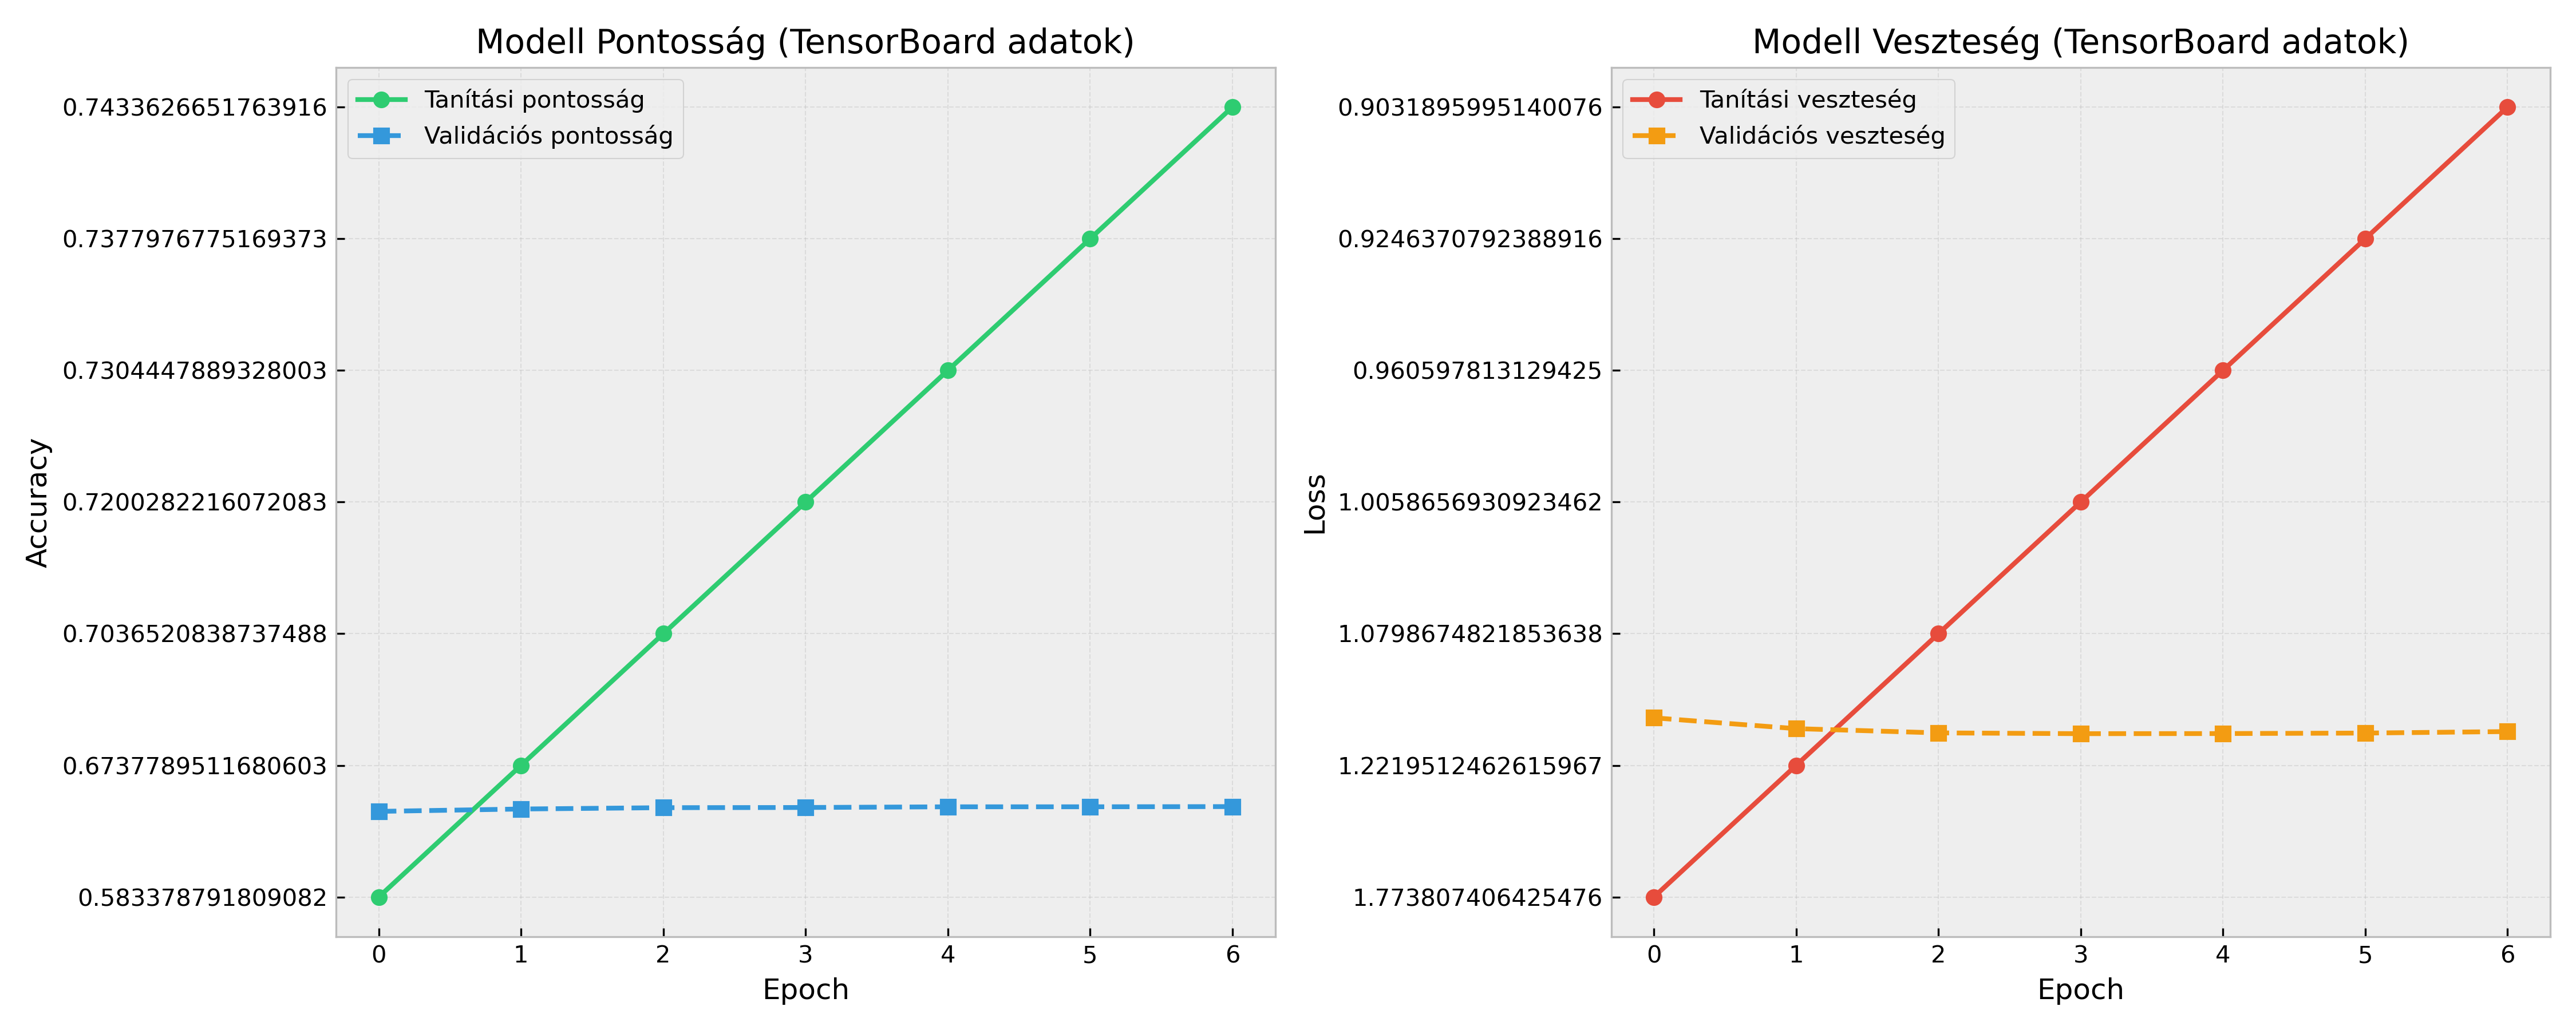
\includegraphics[width=0.95\textwidth]{images/training_curves.png}
    \caption{A modell tanulási folyamatát bemutató pontosság (Accuracy) és veszteség (Loss) görbék.}
    \label{fig:training_curves}
\end{figure}
A modell az első helyes találatot (Top-1 Accuracy) tekintve a teszt halmazon 68,48\%-os pontosságot ért el. Bár ez az érték abszolút skálán nem tűnik kiugrónak, az 594 osztályos besorolási feladat nehézségét és a biológiai taxonómia sajátosságait figyelembe véve valójában kifejezetten jó eredmény. A kiértékelés során elvégzett Top-k analízis rávilágított, hogy a modell \textbf{Top-5 pontossága meghaladja a 90\%-ot}.

\begin{figure}[H]
    \centering
    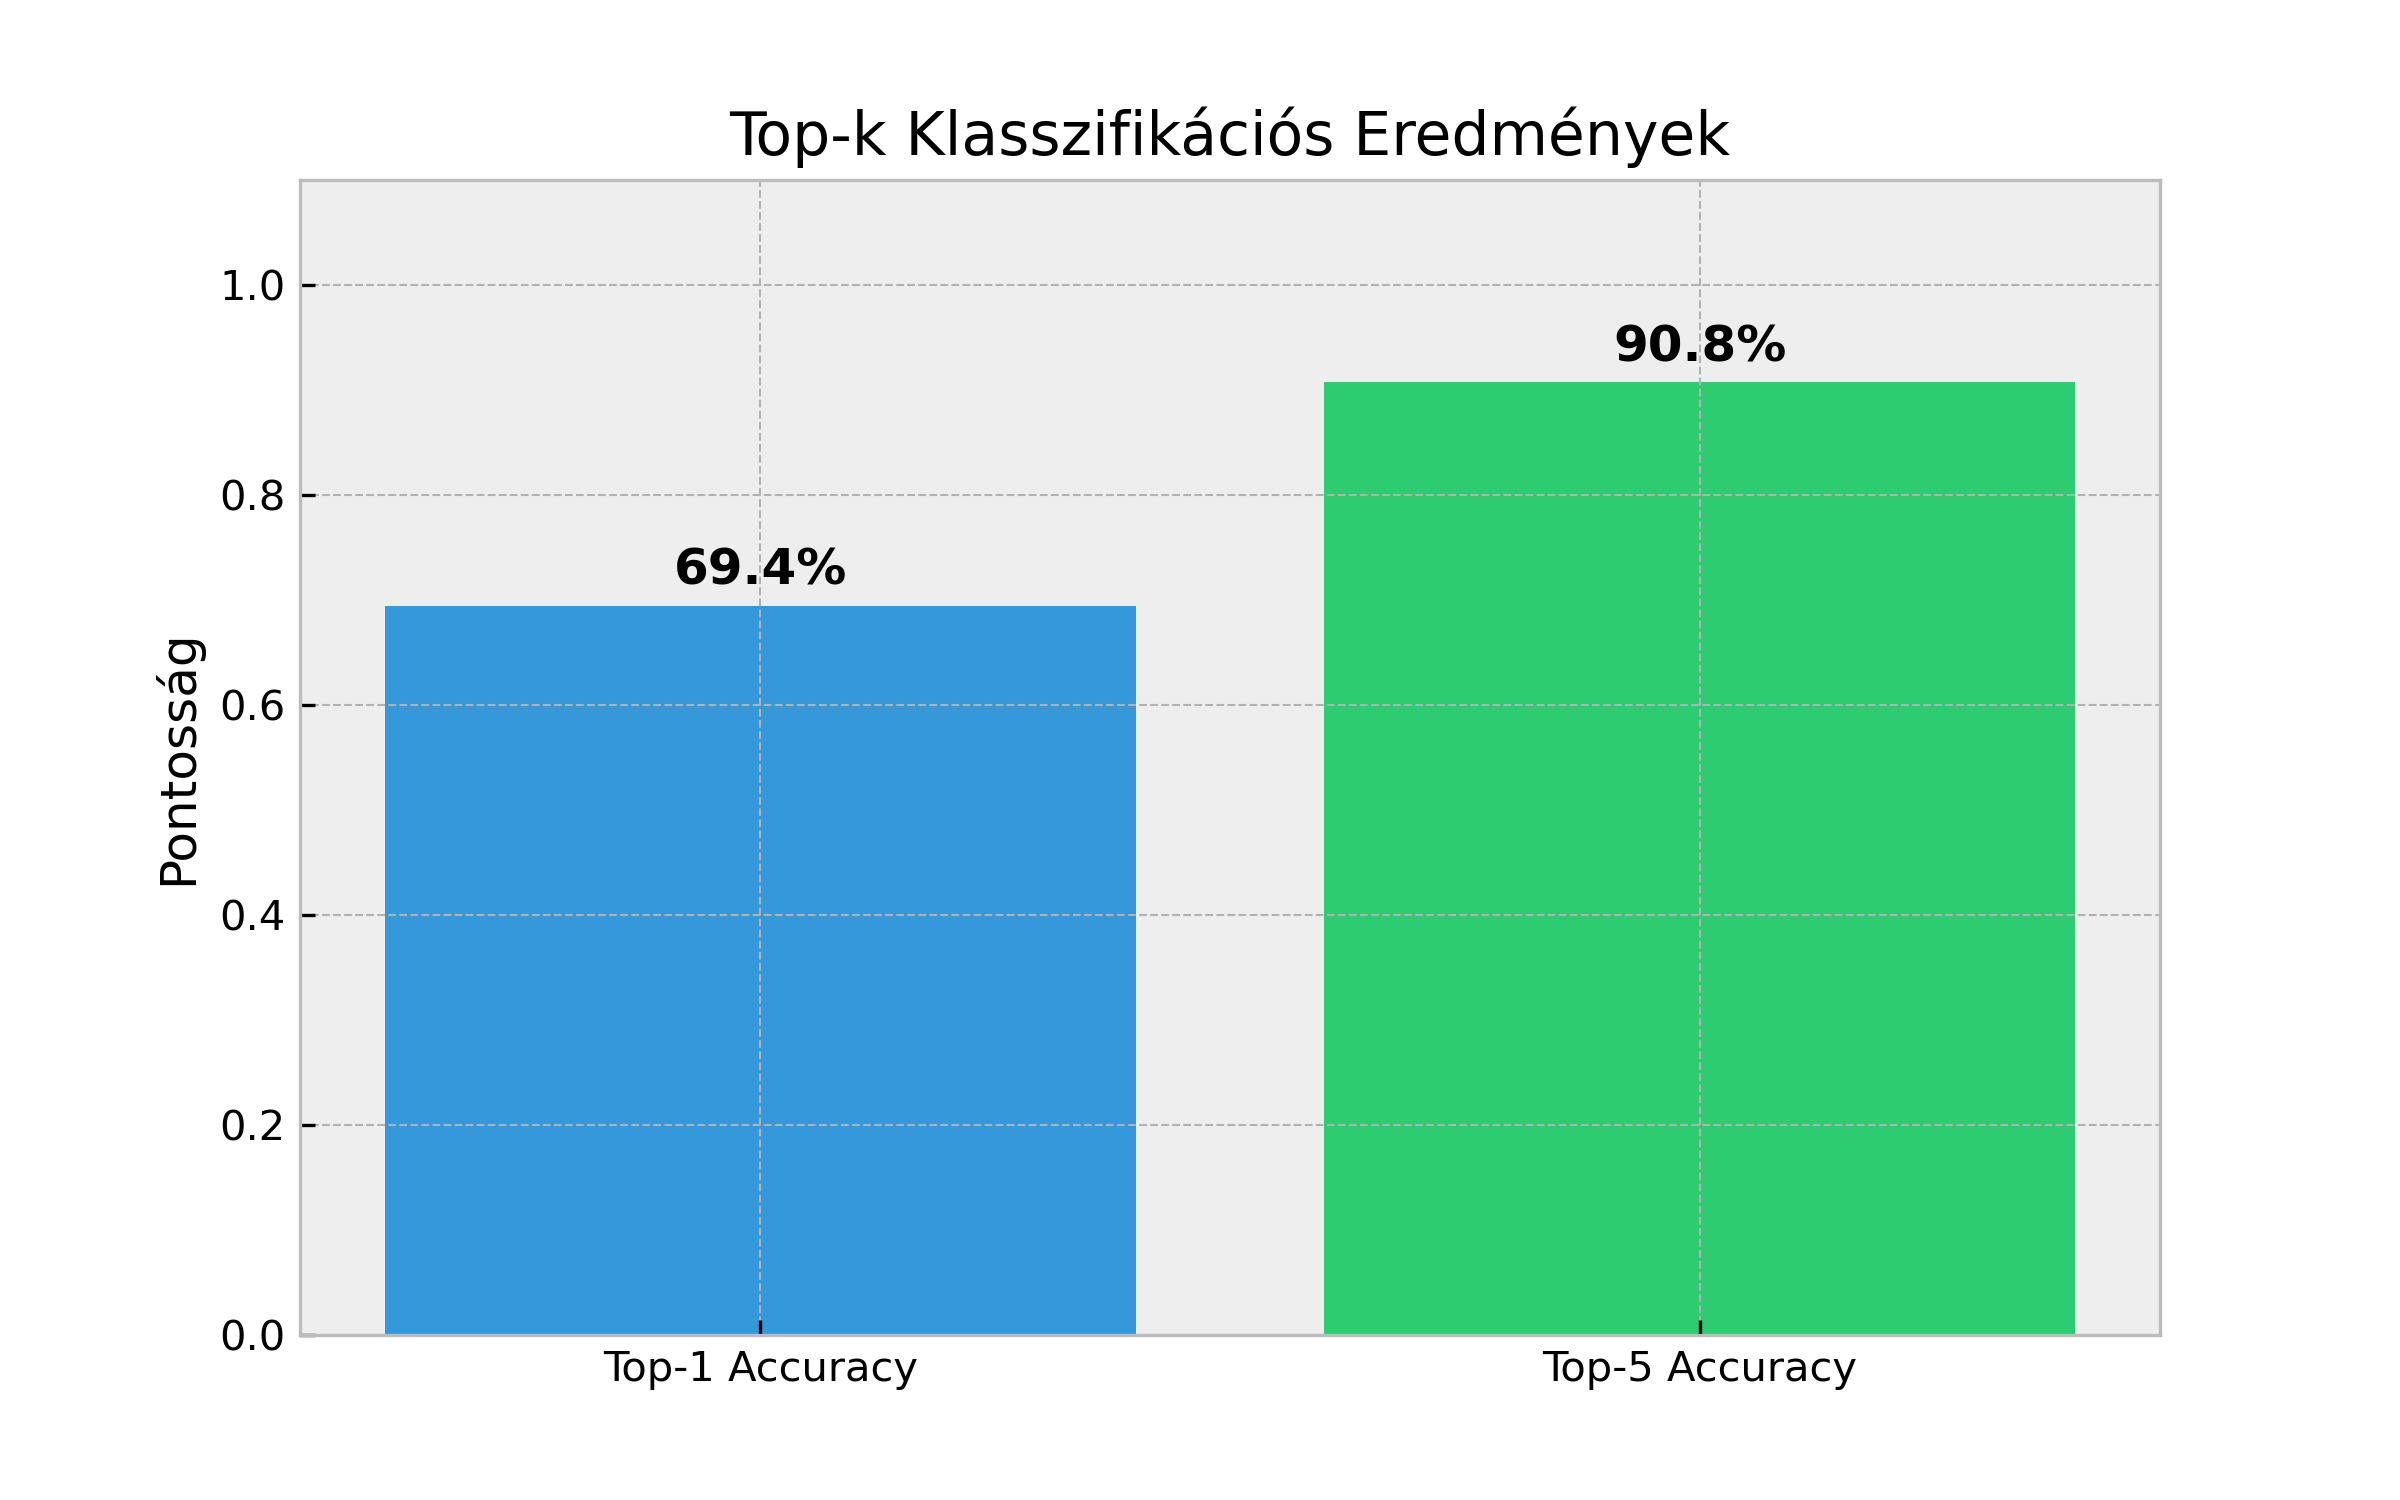
\includegraphics[width=0.85\textwidth]{images/top_k_accuracy.png}
    \caption{A modell Top-1 és Top-5 pontosságának összehasonlítása.}
    \label{fig:topk_accuracy}
\end{figure}

Ez a metrika azt bizonyítja, hogy a hálózat kiválóan képes leszűkíteni a lehetséges jelölteket a megfelelő családra vagy nemzetségre (például biztosan felismeri, hogy a képen egy sirály vagy réce szerepel). A tévesztések döntő többsége kizárólag a morfológiailag szinte azonos, egymással szoros rokonságban álló fajok és alfajok között történik, ahol a vizuális megkülönböztetés még emberi szakértők számára is kihívást jelent.

Ezt a tendenciát a \textit{Larus} (sirályféle) nemzetség 11 fajára elvégzett részletes elemzéssel lehet a legszemléletesebbem bemutatni. A sirályfajok (pl. \textit{Larus argentatus}, \textit{Larus cachinnans}, \textit{Larus michahellis}) morfológiailag rendkívül hasonlóak, és egymástól való megkülönböztetésük tapasztalt ornitológusoknak is kihívást jelent. A \ref{fig:confusion_matrix}. ábrán látható konfúziós mátrix egyértelműen mutatja, hogy a modell szinte sosem téveszti össze a sirályokat teljesen eltérő fajokkal — a tévedések kizárólag a nemzetségen belül, egymáshoz rendkívül közel álló fajok között fordulnak elő.

\begin{figure}[H]
    \centering
    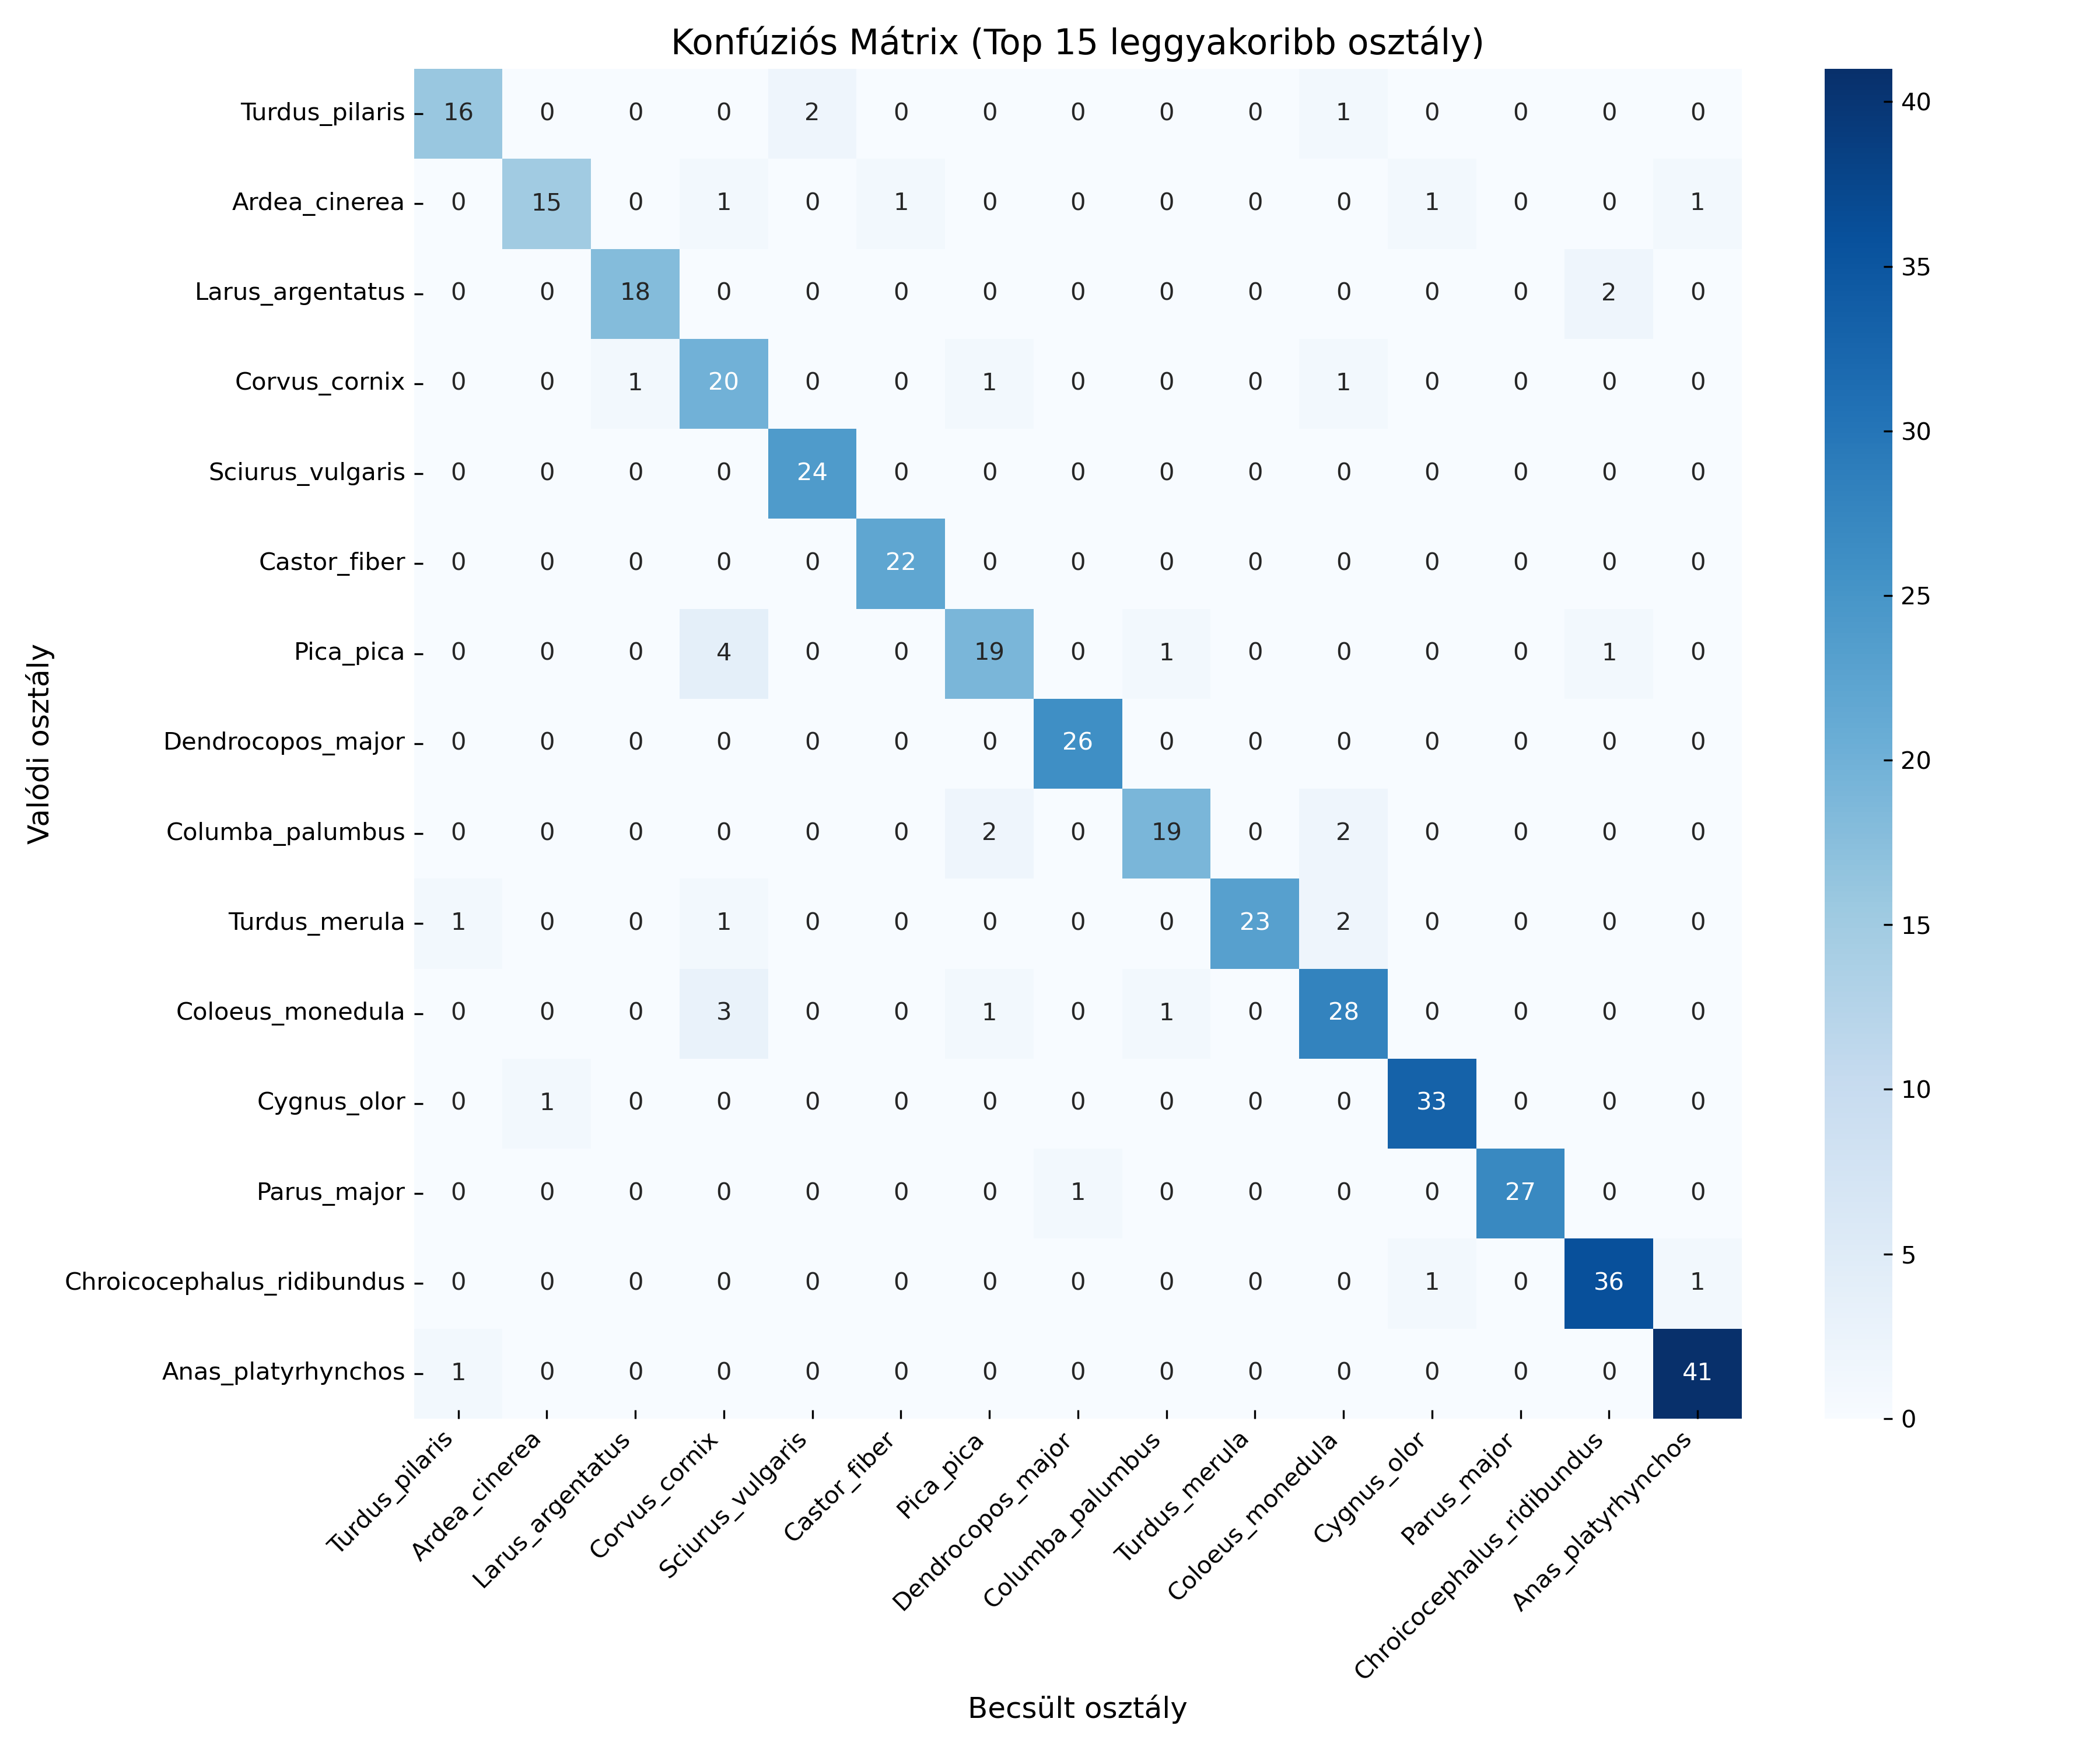
\includegraphics[width=0.95\textwidth]{images/confusion_matrix_top15.png}
    \caption{Konfúziós mátrix a 15 leggyakoribb faj predikciós eredményeiről. Az átló dominanciája jól mutatja, hogy különböző fajok (pl. sirály és őz) között szinte soha nem történik tévesztés.}
    \label{fig:confusion_matrix_top15}
\end{figure}

Összehasonlításképpen a \ref{fig:confusion_matrix}. ábra kizárólag a \textit{Larus} nemzetség 11 fajára fókuszál, ahol a morfológiai hasonlóság miatt a tévesztések jóval hangsúlyosabban jelennek meg.

\begin{figure}[H]
    \centering
    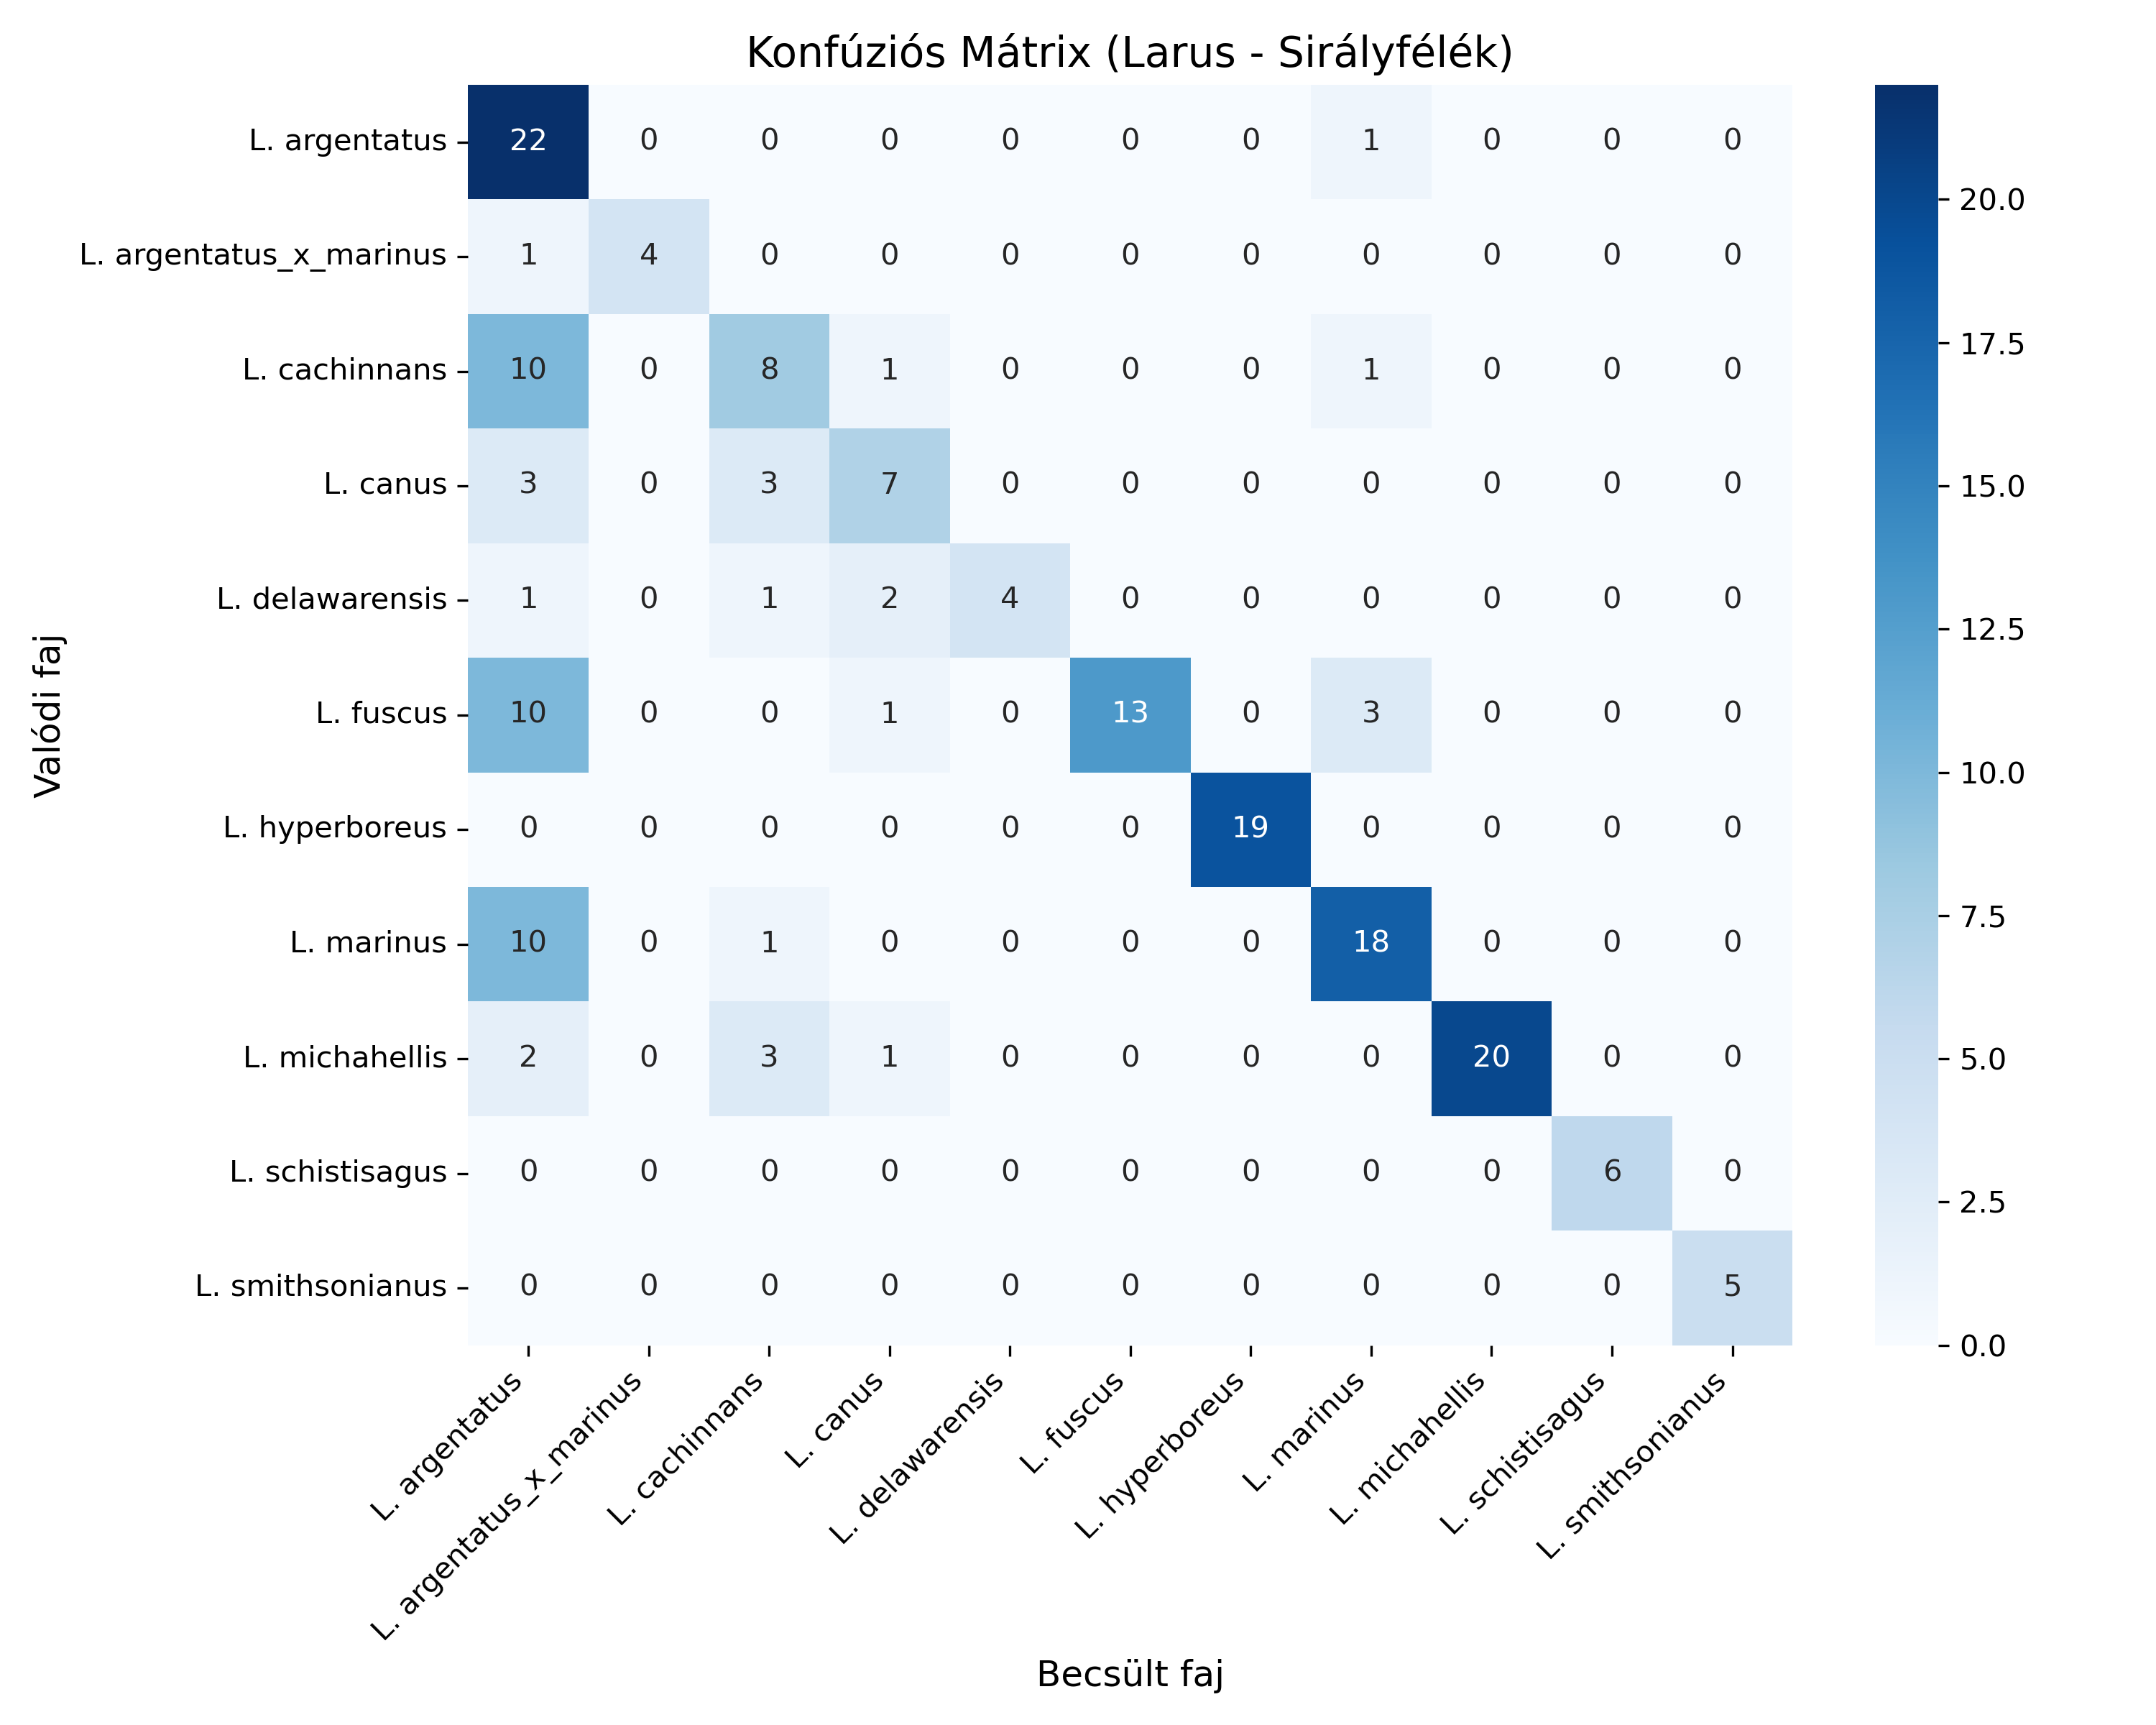
\includegraphics[width=0.95\textwidth]{images/confusion_matrix_subset.png}
    \caption{Konfúziós mátrix a \textit{Larus} (sirályféle) nemzetség 11 fajának predikciós eredményeiről. Az átlón kívüli értékek kizárólag morfológiailag szinte azonos fajok között fordulnak elő.}
    \label{fig:confusion_matrix}
\end{figure}

% ----------------------------------------------------------------------------
\chapter{Tesztelés és Validáció}
\label{ch:test}

Ez a fejezet a szoftver minőségbiztosítási folyamatait, a végrehajtott tesztek típusait, valamint a fejlesztés során szerzett tapasztalatokat és a rendszer skálázhatósági elemzését mutatja be.

\section{Tesztelési terv és Tesztesetek}
A minőségbiztosítás során piramis-modell alapú tesztelési stratégiát alkalmaztam, amely az alacsony szintű egységtesztektől a teljes rendszert átfogó manuális integrációs tesztekig terjed.

\subsection{Modultesztek (Unit Tests) -- Fehérdoboz megközelítés}
A modultesztek célja az egyes izolált függvények és logikai egységek helyességének igazolása. A teszteléshez a \texttt{Pytest} keretrendszer és a \texttt{unittest.mock} könyvtárat használtam, hogy kiiktassam a külső függőségeket (pl. hálózat, adatbázis).

\begin{itemize}
    \item \textbf{Hitelesítési modul (\texttt{test\_auth.py}):}
    \begin{itemize}
        \item \textit{Sikeres regisztráció/bejelentkezés:} Ellenőrzi, hogy a rendszer helyesen dolgozza-e fel a Supabase-től érkező pozitív válaszokat.
        \item \textit{Hibakezelés:} Teszteli az érvénytelen jelszavak, már létező felhasználók és hálózati időtúllépések kezelését.
    \end{itemize}
    \item \textbf{Dashboard logika (\texttt{test\_dashboard\_logic.py}):}
    \begin{itemize}
        \item \textit{Navigációs védelem:} Igazolja, hogy bejelentkezés nélkül a rendszer a \texttt{/login} oldalra irányít.
        \item \textit{Koordináta-kezelés:} Ellenőrzi, hogy a térképes kattintás adatai helyesen konvertálódnak-e numerikus koordinátákká.
        \item \textit{MI inferencia mockolása:} Teszteli az UI frissítését különböző modellkimenetek (fajnevek, konfidencia szintek) esetén, anélkül, hogy a valódi, erőforrás-igényes modellt be kellene tölteni.
    \end{itemize}
\end{itemize}

\subsection{Rendszerteszt és Integrációs tesztelés -- Feketedoboz megközelítés}
A rendszertesztelés során a teljes alkalmazást validáltam a felhasználó szemszögéből, a belső implementáció ismerete nélkül.

\begin{itemize}
    \item \textbf{End-to-End munkafolyamat:} Egy teljes észlelés rögzítése a belépéstől a térképes választáson és feltöltésen át a galériában való megjelenésig.
    \item \textbf{Reszponzivitás ellenőrzése:} A felület használhatóságának tesztelése különböző képernyőméreteken (asztali vs. mobil nézet).
    \item \textbf{Adatkonzisztencia:} Annak ellenőrzése, hogy a Dashboardon végzett műveletek azonnal és helyesen jelennek-e meg a statisztikai modulban és a térképen.
\end{itemize}

\section{Tanulságok és Implementációs változtatások}
A tesztelési fázis során több olyan technikai nehézség merült fel, amely a korábbi tervek módosítását tette szükségessé:

\begin{enumerate}
    \item \textbf{Memóriakezelési problémák:} Az eredeti terv szerint a képeket eredeti felbontásban továbbítottuk volna az MI modellnek. A tesztelés során azonban a Docker konténer gyakran kifogyott a memóriából nagy felbontású fotók esetén. \textbf{Változtatás:} Bevezettem egy azonnali előfeldolgozó lépést, amely $224 \times 224$ képpontra kicsinyíti a fotókat a kliens oldalon, így stabilizálva a rendszer futását.
    \item \textbf{RLS szabályok konfliktusa:} Kezdetben a Row Level Security túl szigorú volt, ami megakadályozta a globális statisztikák (\texttt{user\_stats} tábla) frissítését az észlelések mentésekor. \textbf{Változtatás:} Az adatbázis-sémát és az RLS szabályokat úgy módosítottam, hogy az \texttt{upsert} műveletek engedélyezettek legyenek a hitelesített felhasználók saját rekordjain.
\end{enumerate}

\section{Nagy adattömeg melletti futtatások és Helyesség}
A rendszer skálázhatóságát és megbízhatóságát nagy adathalmazon is vizsgáltam.

\begin{itemize}
    \item \textbf{Modell validáció:} A tanítás során használt 170\,195 képből álló adathalmazon a hálózat 68,48\%-os Top-1 pontosságot ért el. Az eredmények elemzésekor megállapítható, hogy a tévedések nagy része vizuálisan nagyon hasonló fajok (pl. különböző őzfajok) között történt, ami a feladat nehézségét tükrözi.
    \item \textbf{Adatbázis terhelés:} Szimuláltam több ezer észlelés egyidejű tárolását. A Supabase (PostgreSQL) és a PostgREST interfész stabilan kezelte a nagy adatmennyiséget, a lekérdezési idők a galéria nézetben 200 ms alatt maradtak az indexelt \texttt{user\_id} mezőnek köszönhetően.
\end{itemize}

\section{Hatékonyság és Skálázhatósági elemzés}
A szoftver futási hatékonysága és jövőbeli bővíthetősége kulcsfontosságú.

\begin{itemize}
    \item \textbf{Futási hatékonyság:} Egy átlagos kép osztályozása (beolvasás + inferencia + DB mentés) körülbelül 1.2--1.8 másodpercet vesz igénybe CPU környezetben. GPU támogatással (pl. \texttt{tensorflow-gpu} konténerben) ez az idő 100 ms alá szorítható.
    \item \textbf{Horizontális skálázhatóság:} Mivel a Dashboard alkalmazás alapvetően állapotmentes (a munkamenetet a \texttt{dcc.Store} kezeli a böngészőben), a \texttt{wildlife-dashboard} konténerből könnyen futtatható több példány egy terheléselosztó (pl. Nginx) mögött.
    \item \textbf{Adatbázis skálázhatóság:} A helyileg futó PostgreSQL adatbázis erőforrásai a Docker konfiguráción keresztül skálázhatók. Szükség esetén a rendszer migrálható a Supabase Cloud felhőalapú infrastruktúrájára is, ami automatikus vízszintes skálázást tenne lehetővé.
\end{itemize}

\section{A szoftver értékelése}
A szoftver futtatása és a tesztelési fázis tapasztalatai alapján az alábbi értékelést adhatjuk a rendszer minőségéről.

\subsection{Helyesség és Megfelelőség}
A program teljes mértékben megfelel a feladat-meghatározásban és a rendszertervben rögzített elvárásoknak. A funkcionális tesztek igazolták, hogy:
\begin{itemize}
    \item A képfeltöltés és az automatikus MI-alapú osztályozás hiba nélkül zajlik.
    \item Az észlelések földrajzi adatai pontosan tárolódnak és jelennek meg a térképen.
    \item A statisztikai adatok valós időben frissülnek a felhasználói interakciók hatására.
\end{itemize}

\subsection{Robusztusság és Hibatűrés}
A szoftver tervezésekor kiemelt figyelmet fordítottam a felhasználói hibák kezelésére és a rendszerszintű stabilitásra:
\begin{itemize}
    \item \textbf{Hibatűrés:} A rendszer védett az érvénytelen bemenetek ellen (pl. hiányzó koordináta esetén nem omlik össze, hanem figyelmezteti a felhasználót). A hálózati és adatbázis-hibák kezelése \texttt{try-except} blokkokkal és felhasználóbarát hibaüzenetekkel történik.
    \item \textbf{Életszerű működés:} A rendszer nagy mennyiségű (több száz) észlelés tárolása és megjelenítése esetén is hatékony marad, köszönhetően az adatbázis-oldali indexelésnek és a Dash reaktív frissítési mechanizmusának.
    \item \textbf{Stabilitás:} A Docker-alapú izoláció garantálja, hogy a rendszer „jóindulatú” tesztelés (szabványos használat) mellett stabil maradjon, elkerülve a váratlan leállásokat.
\end{itemize}

\subsection{Felhasználó-barátság és Ergonómia}
Az alkalmazás felülete modern, esztétikus és a szakterületi igényekhez igazodik:
\begin{itemize}
    \item \textbf{Esztétika:} A „Glassmorphism” stílus, a sötét mód (Dark Mode) és a harmonikus színpaletta (Inter fontcsalád, zöld és kék gradiensek) prémium megjelenést és kényelmes használatot biztosít alacsony fényviszonyok (pl. éjszakai terepmunka) mellett is.
    \item \textbf{Áttekinthetőség:} Az SPA (Single Page Application) megközelítés és a tiszta navigációs sáv révén a funkciók könnyen elérhetők. A térképes interakciók intuitívak, követik a modern webes tradíciókat.
    \item \textbf{Súgó és Tájékoztatás:} A rendszer az intuitív felépítése miatt nem igényel külön súgó menüt; a felhasználót a felületen elhelyezett kontextuális instrukciók és egyértelmű feliratok vezetik végig a folyamaton (pl. a feltöltés előtti útmutatók), a kritikus műveletek közben pedig betöltési indikátorok tájékoztatnak a folyamat állapotáról.
    \item \textbf{Nyelvezet:} A feliratok konvencionális magyar nyelvűek, kerülik a szakmai zsargont ott, ahol ez nem indokolt, biztosítva az egyértelműséget.
\end{itemize}

% ----------------------------------------------------------------------------
\chapter{Összefoglalás}
\label{ch:sum}

A szakdolgozat keretében egy olyan komplex rendszert sikerült létrehozni, amely választ ad a modern természetvédelmi kutatások kihívásaira. A Dash keretrendszer, a Supabase infrastruktúra és a ConvNeXt neurális hálózat kombinációja egy robusztus, mégis könnyen kezelhető platformot eredményezett.

A jövőben a rendszert további funkciókkal, például automatikus EXIF-adat kinyeréssel és real-time videóanalízissel lehetne bővíteni, tovább segítve a vadon élő állatok védelmét.

% ----------------------------------------------------------------------------
\printbibliography[title=\biblabel]

\end{document}
